% !TeX encoding = UTF-8
% !TeX program = pdflatex
% !TeX spellcheck = it\_IT
\documentclass[binding=0.6cm, oneside, noexaminfo, italian]{sapthesis}
\usepackage[italian]{babel}
\usepackage[utf8]{inputenc}
\usepackage{hyperref}
\usepackage{graphicx}
\usepackage{afterpage}
\usepackage{makeidx}
\usepackage{chngcntr}
\counterwithin{figure}{section}

\renewcommand{\thesection}{\arabic{section}}
\makeindex
\newcommand\blankpage{%
    \null
    \thispagestyle{empty}%
    \addtocounter{page}{-1}%
    \newpage}


\title{4Money}

\subtitle{Gestisci il tuo portafoglio in maniera smart}

\author{Cristian Andrei Mai Mihai}

\IDnumber{1942925}

\course{Corso di Laurea in Ingegneria Informatica e Automatica}

\courseorganizer{Facoltà di Ingegneria dell'informazione, informatica e statistica}

\AcademicYear{2022/2023}

\advisor{Prof. Riccardo Rosati}

\customadvisorlabel{Relatore}

\copyyear{2023}

\authoremail{cristianmm1240@gmail.com}

\begin{document}

\frontmatter
\maketitle

\afterpage{\blankpage}

\newpage

\tableofcontents

\mainmatter
\newpage

\section{Introduzione}
\subsection{Presentazione}
Questa tesi ha lo scopo di presentare 4Money, un’applicazione web nata come progetto del corso di Linguaggi e Tecnologie per il Web, descrivendo le funzionalità di tale sito sia lato client che lato server, oltre alle motivazioni che hanno portato alla scelta di certe implementazioni. \\ \\
4Money è un’applicazione web che si pone l’obiettivo di aiutare i propri utenti a gestire al meglio le proprie finanze e per raggiungerlo offre un’interfaccia interattiva e funzionale la quale consente all’utente una vasta varietà di azioni disponibili e funzioni:
\begin{itemize}
    \item Conserva informazioni riguardanti le spese o gli introiti salvati dall’utente in base a specifiche categorie, sia che questi siano passati o futuri;
    \item Permette di gestire un fondo di risparmio, detraendo o assegnando a esso risorse in base alle necessità dell’utente;
    \item Presenta diversi grafici per aiutare a visualizzare in modo rapido e intuitivo le proprie abitudini finanziarie, dalla quantità di soldi che vengono spesi durante i vari mesi dell’anno, alla percentuale per categoria delle spese del mese corrente;
    \item Completa libertà nella gestione del proprio profilo;
    \item Possibilità di esportare i dati dei propri movimenti in vari formati;
\end{itemize}
Sono presenti, inoltre, tre profili di tipo amministratore, uno per ognuno dei creatori di 4Money, per una gestione di dinamica degli utenti e delle categorie delle transazioni. In particolare, gli amministratori possono bloccare o, se ritenuto necessario, eliminare gli account degli utenti comuni; vi sono dei grafici a loro dedicati per osservare le distribuzioni degli iscritti alla piattaforma in base a diversi tipi di dati; infine è concesso loro creare, eliminare o modificare le categorie delle transazioni.
\subsection{Tecnologie utilizzate}
4Money è stato realizzato utilizzando le classiche tecnologie per quanto riguarda la creazione di web app, a cui sono state aggiunte particolari librerie per sviluppare alcune funzionalità chiave del sito. \\ \\
In primis è stato utilizzato Html, o HyperText Markup Language, un linguaggio di markup che ha il compito di fungere da struttura portante di qualsiasi pagina web. Gli ipertesti generati con Html sono documenti contenenti testo, immagini, audio, video o collegamenti ipertestuali, ovvero riferimenti ad altri documenti o altre pagine web stesse. La sintassi di Html sfrutta essenzialmente il concetto di "tag", il quale permette di marcare parti di testo dando loro particolari caratteristiche, modificabili attraverso degli attributi specifici del rispettivo tag. \\ \\
Per quanto riguarda lo stile sono stati utilizzati Css e Bootstrap. Il primo, il cui acronimo sta per Cascading Style Sheets, è un linguaggio per la realizzazione di fogli di stile, che sfrutta i tag di Html per la propria implementazione. I fogli di stile possono essere di vari tipi, ma per questo progetto è stato utilizzato un Css esterno, ovvero un file che definisce le scelte stilistiche, importato dalle pagine al momento della loro creazione. In particolare, 4Money presenta solo un foglio per tutte le pagine, per rendere lo stile comune a ognuna di loro. Bootstrap, invece, è un framework Css tra i più utilizzati per lo sviluppo di front-end, che sfrutta a sua volta codici Html, Css e JavaScript per implementare diversi oggetti utili nella creazione di interfacce web, senza dover cambiare la sintassi dei linguaggi su cui si basa. \\ \\
Per la dinamicità del sito lato client è stato utilizzato JavaScript, un liguaggio ad oggetti, interpretato e di alto livello, che è a sua volta può trovarsi in file apparte o immerso nel codice Html; nel caso specifico di 4Money si trovano entrambe le strutture. Gli script creati con questo linguaggio vengono eseguiti al momento dell'apertura della pagina alla quale appartengono. \\ \\
Le funzioni logiche del lato server sono state implementate con Php, uno dei più popolari sistemi di scripting per back end nello sviluppo di web app. \MakeUppercase{è} un linguaggio interpretato, di alto livello e anch'esso immergibile nel codice Html, che permette di rendere le pagine web dinamiche e di farle interagire efficacemente con il database. \\ \\
Per la base di dati e la comunicazione con questa sono stati utilizzati SQL e Json. Il primo è un linguaggio che permette di interagire direttamente con il database sfruttando il concetto di "query", un sistema di richieste per la selezione di dati depositati in base a specifiche caratteristiche; il secondo, detto anche JavaScript Object Notation, rappresenta il formato standard per la serializzazione e la de-serializzazione di oggetti Javascript, ovvero la conversione da oggetto a stringa e viceversa. \\ \\
4Money utilizza anche tecnologie quali AJAX, o Asynchronous Javascript And XML; basato su JavaScript, ha lo scopo di implementare interazioni asincrone tra web client e web server, ovvero permette di non dover caricare nuovamente la pagina per piccoli cambiamenti, ottenendo così una maggiore velocità di esecuzione e visualizzazione delle pagine. \\ \\
I numerosi grafici presenti nel sito sono invece stati implementati con Highcharts, una libreria online costruita su JavaScript e TypeScript utilizzabile su ogni tipo di linguaggio, offrendo un vasto numero di strumenti per personalizzare al meglio la propria esperienza grafica. Un maggiore approfondimento sulla sintassi e invocazione di Highcharts verrà affrontato in seguito durante la spiegazione di uno dei codici.

\newpage
\section{Lato Client}
Questa sezione si occuperà di descrivere le varie componenti delle pagine visualizzabili di 4Money, illustrando le motivazioni che hanno portato alla scelta di certe implemenazioni e le loro funzionalità. Nella prima parte verranno discusse le parti comuni a tutti i tipi di utenti e a quelli comuni, per poi passare alla trattazione dei profili di tipo amministratore. Tutti i dati reletivi agli account sono stati fittizi e creati dall'autore per rendere più comprensibile come le pagine funzionino e il loro aspetto nel caso di un account attivo ed utilizzato.
\subsection{La NavBar}
Prima di iniziare a descrivere le pagine vere e proprie è utile trattare prima la barra di navigazione, a cui ci riferiremo in questa tesi con il termine "navbar". \\
La navbar è un sistema attraverso il quale è possibile navigare tra le varie pagine del sito a seconda del tipo di autorizzazione di cui l'utente dispone. Esistono infatti tre diverse istanze di questa: una per l'utente che non ha effettuato l'accesso, una per gli utenti comuni e infine una per gli utenti amministratori.
Nonostante queste divisioni, tutti i tipi hanno una struttura comune, che si basa su tecnlogie quali Html per la struttura, Css e Bootstrap per la forma e Php per la scelta di che tipo di navbar vada mostrata in base ai dati della sessione in corso, oltre a funzione che la rendono dinamica. \\
\begin{figure}[h]
    \centering
    
\includegraphics[width=1\linewidth]{navbar_logout.png}
    \caption{Navbar utente che non ha effettuato l'accesso}
    \label{fig:navbar_logout}
\end{figure} \\
La navbar sovrastante è quella visualizzata quando non si è effettuato nessun tipo di accesso. Sono presenti cinque pulsanti di indirizzamento verso le rispettive pagine. Da sinistra verso destra abbiamo:
\begin{itemize}
    \item Un'icona che riporta il nome del sito e indirizza verso la pagina "Home"
    \item Il pulsante "Home" che come il precedente porta verso l'omonima pagina
    \item Il pulsante "Informazioni" che porta verso l'omonima pagina, non trattata in questa relazione in quanto riporta solamente informazioni sui creatori dell'applicazione e perciò considerata non di interesse
    \item Il pulsante "Accedi" che porta verso la pagina "Login" per poter effettuare l'accesso
    \item Il pulsante "Registrati" che porta verso la pagina "Register" per poter effettuare la registrazione
\end{itemize}
Da notare il fatto che nel caso della figura 2.1 il pulsante "Home" presenta una forma differente rispetto al vicino; questa è una caratteristica della navbar, la quale "illumina" in arancio il pulsante relativo alla pagina in cui ci si trova, rendendolo anche inattivo. Ciò sarà ovviamente riscontrabile anche nelle successive navbar. \\
\begin{figure}[h]
    \centering
    
\includegraphics[width=1\linewidth]{navbar_utente.png}
    \caption{Navbar utente comune}
    \label{fig:navbar_utente}
\end{figure} \\
Questa navbar presenta elementi simili alla precedente, ma si notano cambiamenti riguardo alle pagine a cui si può accedere ora. La parte destra di questa presenta invece maggiori differenze: al posto dei pulsanti per accedere o registrarsi vi sono altri che presentano il nome di "LEMEMIHE3" e "Logout". Il primo è relativo alla pagina del profilo e il suo nome è quello dell'username dell'utente, mentre il secondo consente di disconnettere l'account. \\
\begin{figure}[h]
    \centering
    
\includegraphics[width=1\linewidth]{navbar_admin.png}
    \caption{Navbar utente amministratore}
    \label{fig:navbar_admin}
\end{figure} \\
Infine la navbar degli amministratori, la quale permette di accedere a pagine loro esclusive, ma anche ad altre simili quali utente nel caso del pulsante "CRISTIAN", il quale riporta il nome del proprietario di questo account di tipo amministratore, e quello di "Logout".
\newpage
\subsection{Home}
\begin{figure}[h]
    \centering
    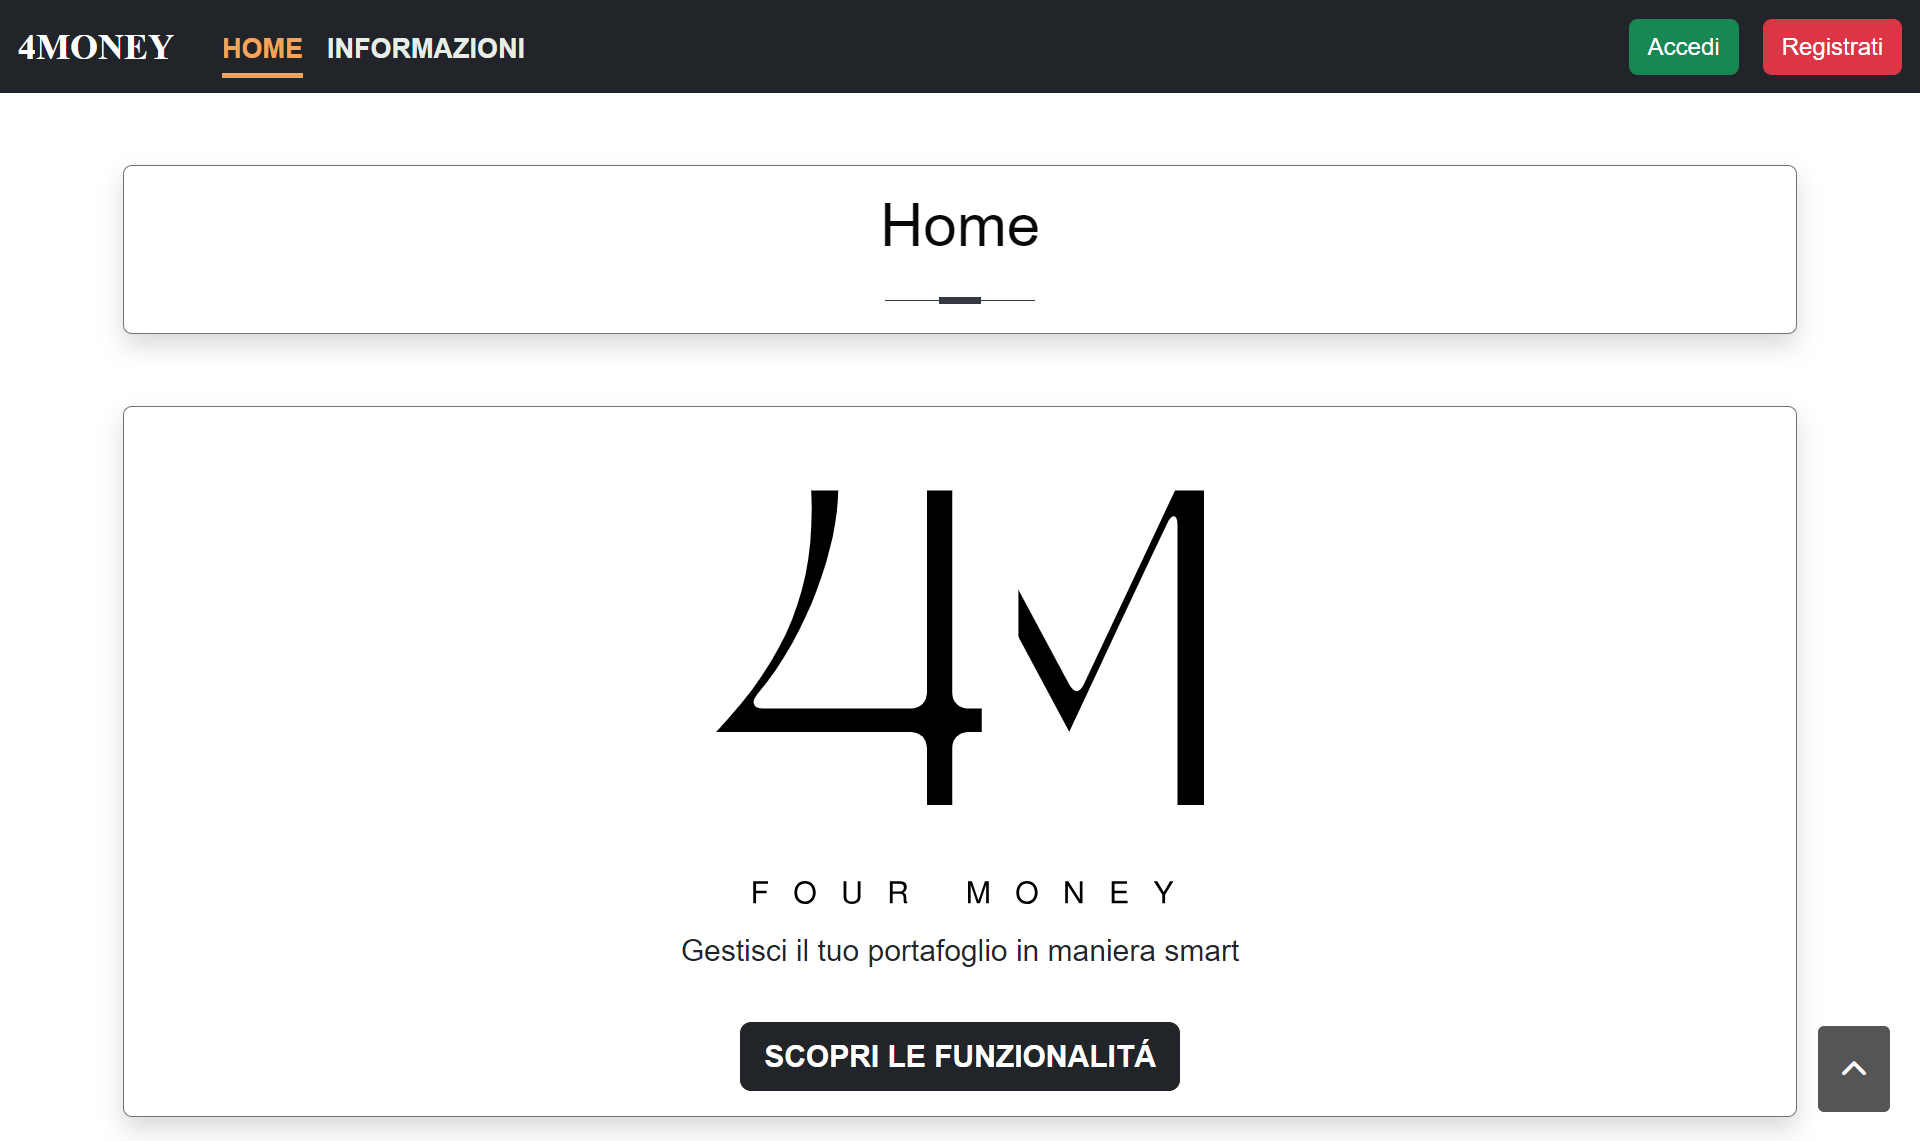
\includegraphics[width=1\linewidth]{home_base.png}
    \caption{Pagina Home}
    \label{fig:home}
\end{figure}
La pagina "Home" è la pagina che funge da "index" dell'applicazione. Le principale funzioni che questa offre sono quelle di facciata per poter passare alle altre pagine attraverso la navbar. Inoltre è presente un pulsante "Scopri le funzionalità" che consente di aprire un sipario come si può vedere nella figura 2.5. La pagina presenta ora le principali funzionalità di 4Money allegando vicino a una rapida descrizione di queste un'immagine esemplificativa. Lo scopo è quello di presentare l'applicazione ai nuovi utenti facendo loro scoprire ciò che possono fare.
\begin{figure}[!ht]
    \centering
    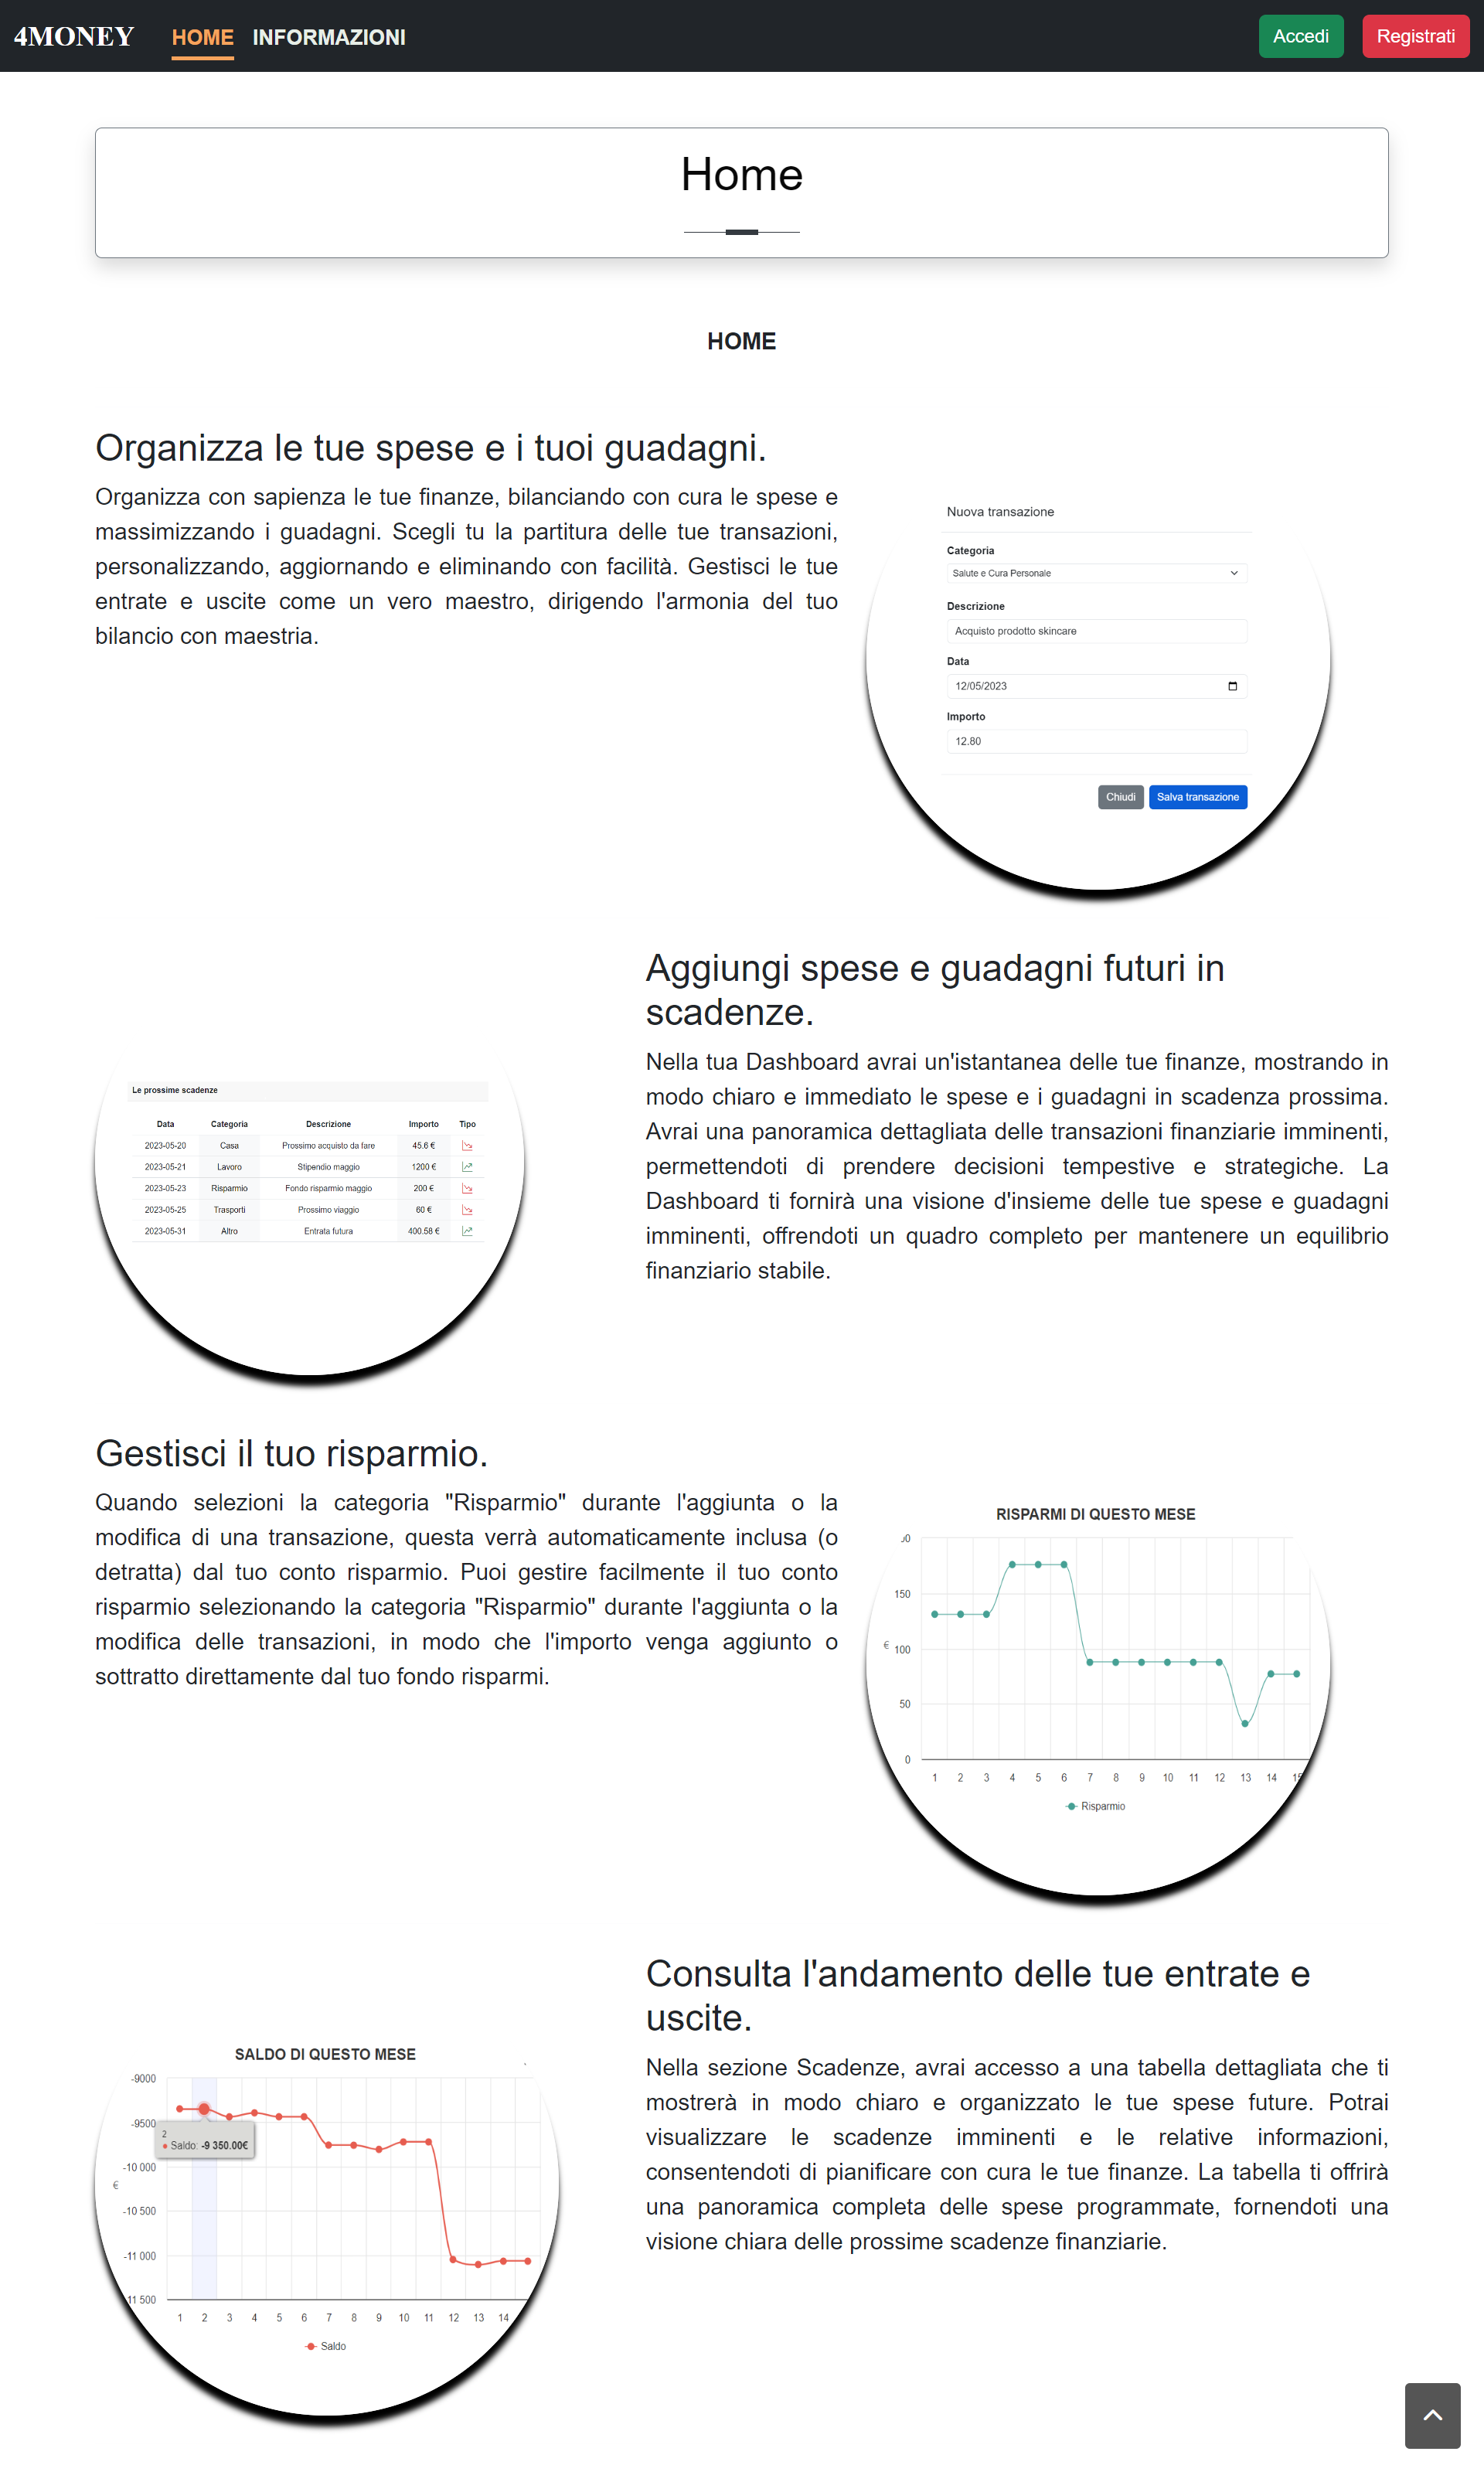
\includegraphics[width=0.9\linewidth]{home2.png}
    \caption{Home sipario}
    \label{fig:home_sipario}
\end{figure}
\newpage
\subsection{Register}
\begin{figure}[h]
    \centering
    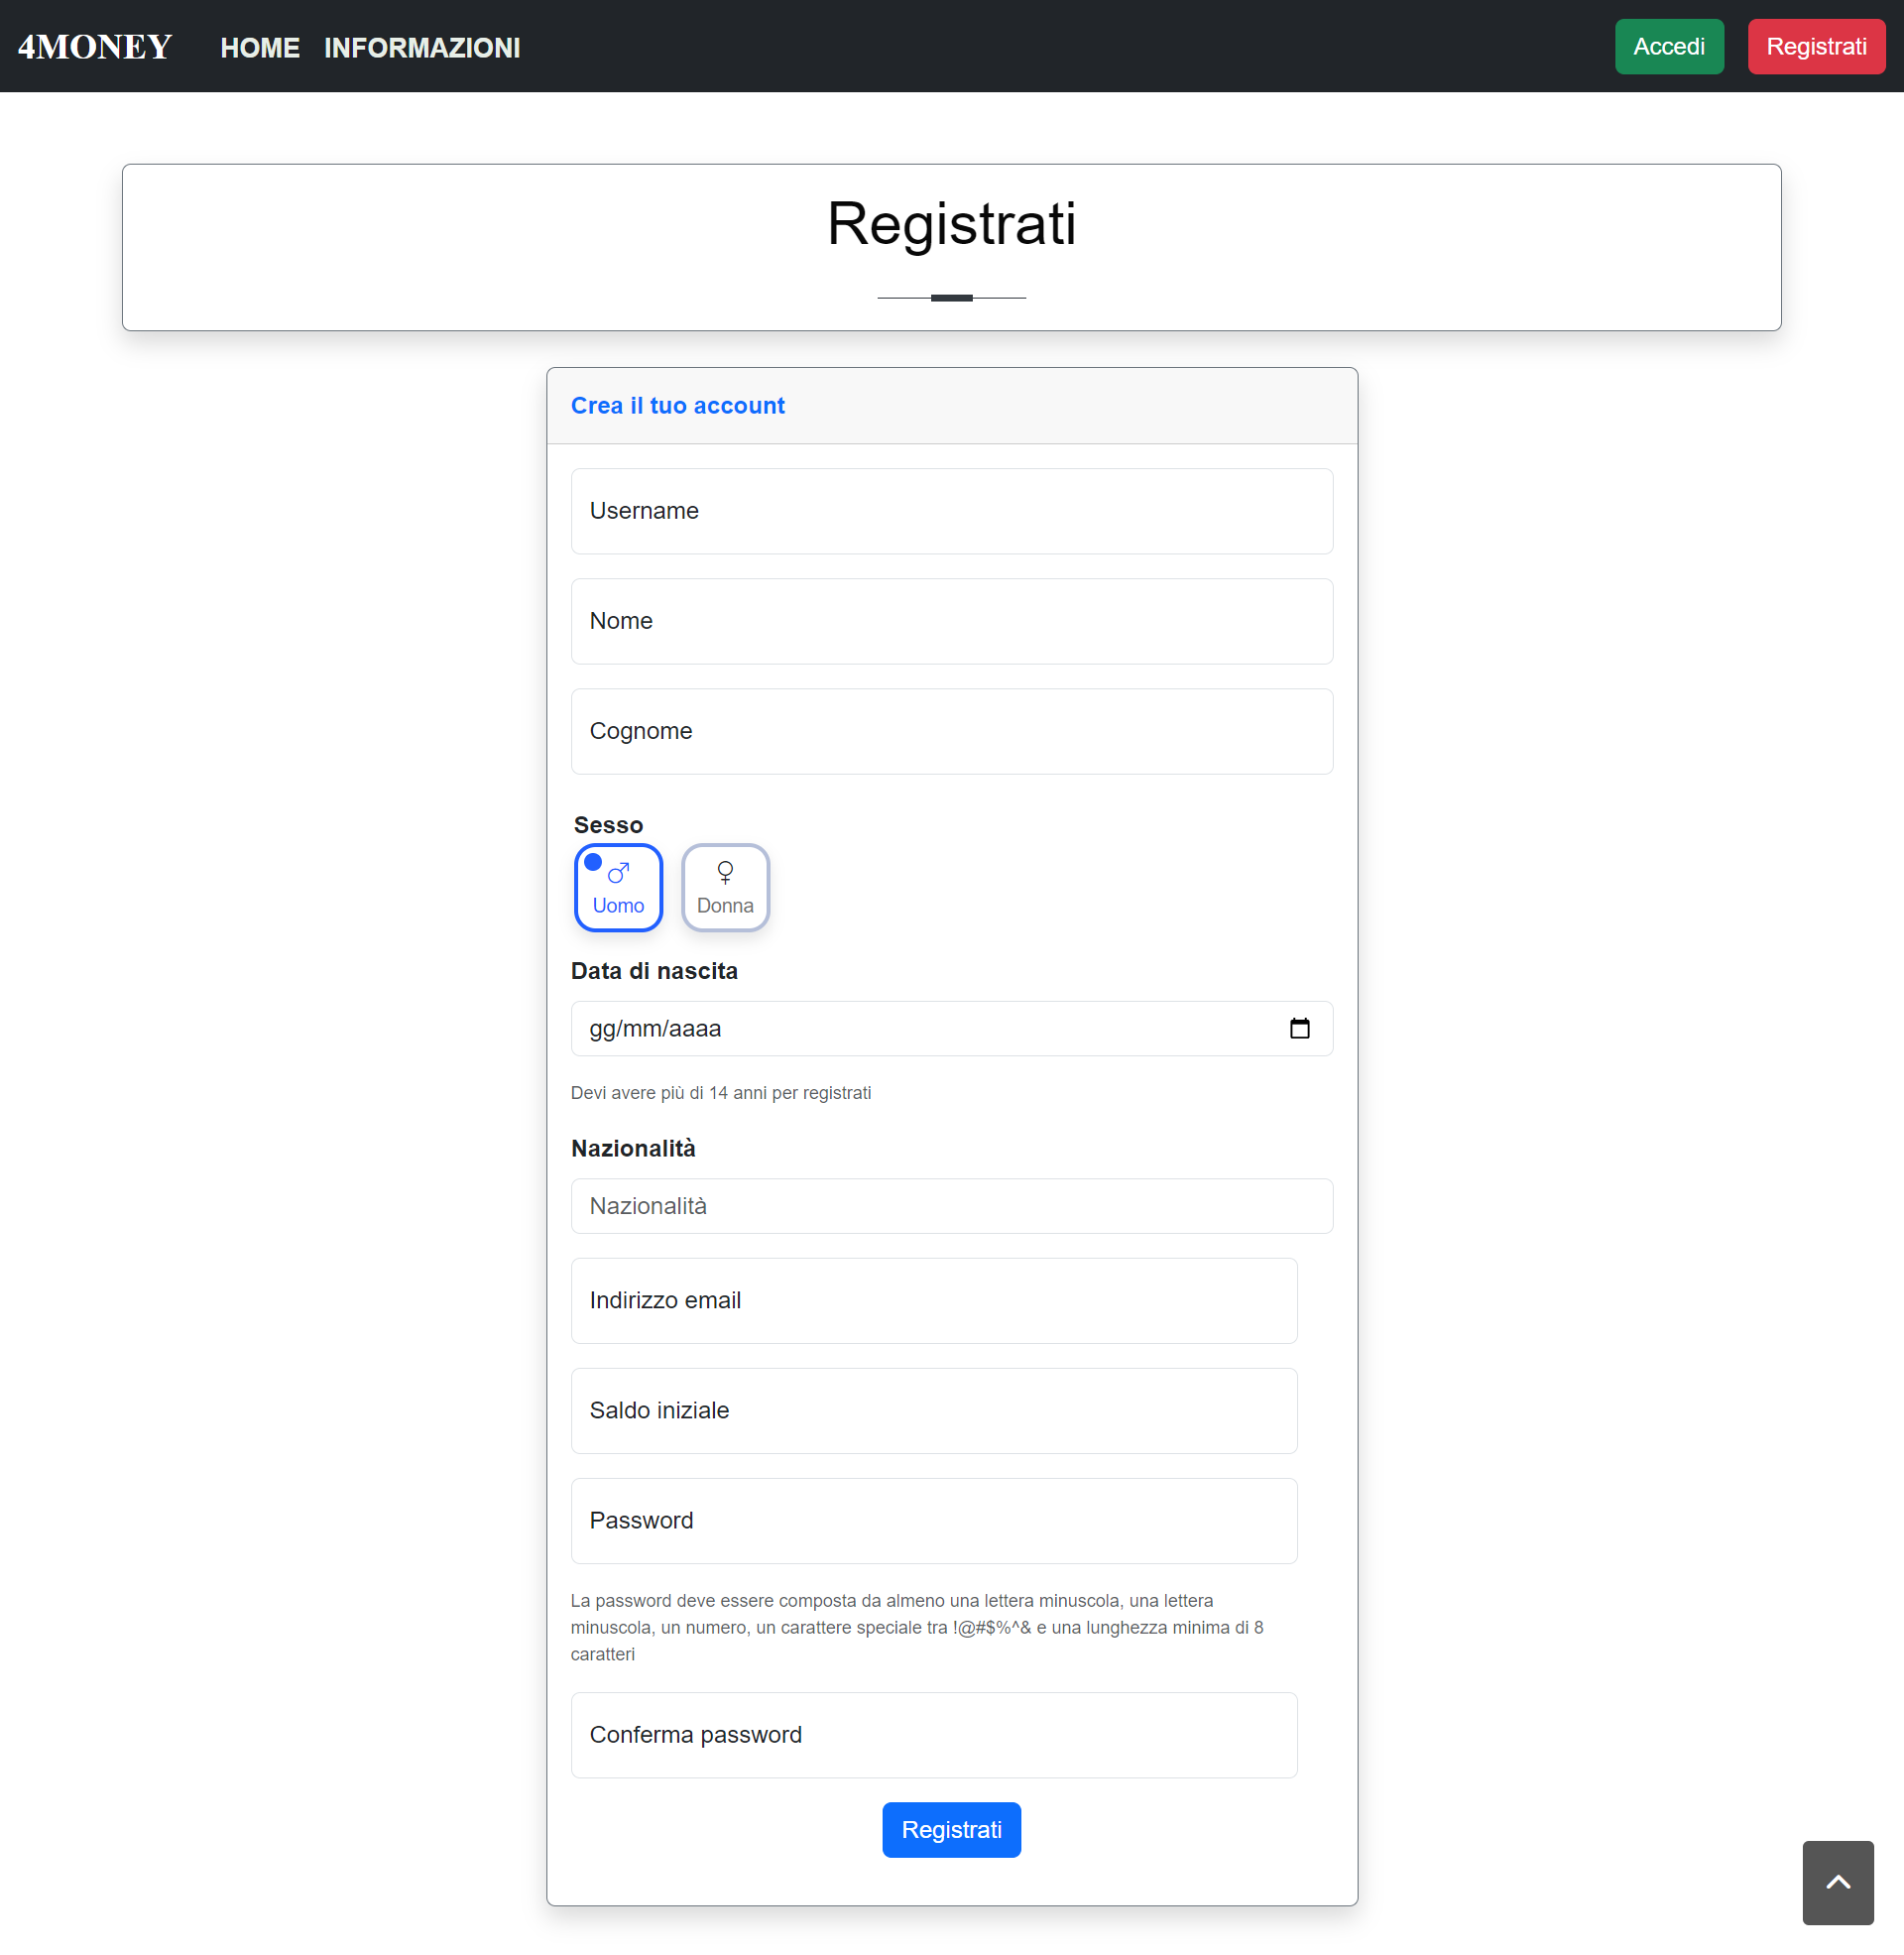
\includegraphics[width=1\linewidth]{register.png}
    \caption{Pagina di registrazione}
    \label{fig:register}
\end{figure}
La pagina "Register" è dedicata alla registrazione degli utenti, i quali dovranno inserire i dati loro richiesti secondo un formato prestabilito. Queste informazioni possono essere personali, come nome e cognome, o relative all'account stesso come username, password o saldo iniziale. I campi compilati hanno inoltre dei prerequisiti per essere convalidati, alcuni dei quali sono mostrati sotto il rispettivo campo come nel caso della password. La convalida avviene in più modi: in modo dinamico utilizzando JavaScript durante la compilazione dei singoli campi, mostrando un segnale di errore nel caso non venga rispettato il formato richiesto, come per esempio l'inserimento di un numero nel campo "Nome" oppure selezionare una data di nascita per cui l'utente avrebbe un'età inferiore ai 14 anni; se viene comunque inviato il "form", ovvero il modulo in Html, nonostante gli errori usando il pulsante "Registrati", avverrà un nuovo controllo sui campi sia lato Client con JavaScript, sia lato server con Php. Il controllo lato Server è necessario per la verifica in quanto il controllo lato Client potrebbe semplicemente essere eluso eliminando le righe di codice JavaScript che lo effettua; a suo modo quest'ultimo ha il compito di facilitare il compito del Server, effettuando una prima verifica e bloccando la registrazione se necessario, in modo che il Server non debba analizzare campi sbagliati. Il tipo di account che è possibile creare in questa pagina è quello comune, mentre gli account di tipo amministratore non possono essere creati, se non inserendoli direttamente nella base di dati.
\subsection{Login}
\begin{figure}[h]
    \centering
    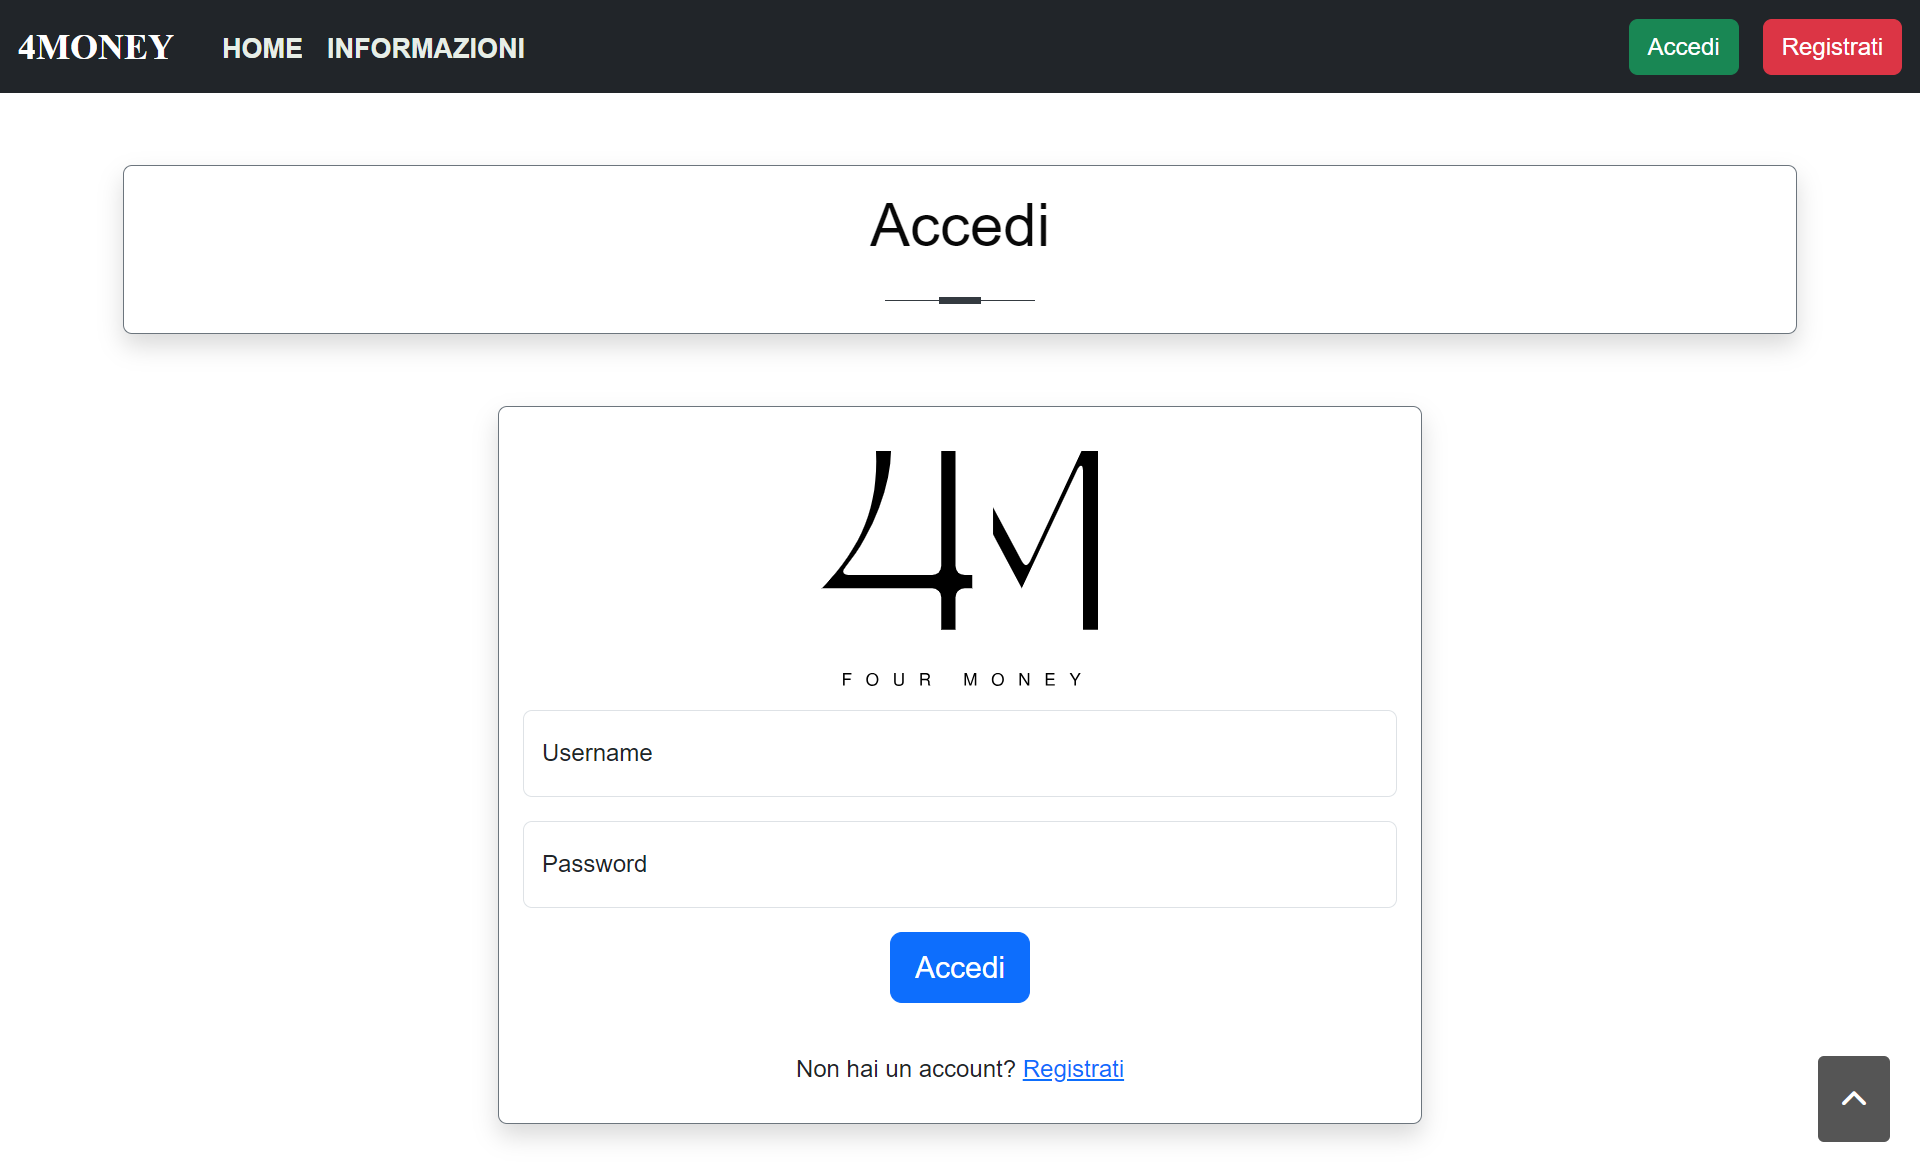
\includegraphics[width=1\linewidth]{login.png}
    \caption{Pagina di accesso}
    \label{fig:login}
\end{figure}
La pagina "Login" è dedicata all'accesso degli utenti. I dati richiesti vanno inseriti nei rispettivi campi, implementati dentro un form Html in modo simile alla pagina "Register", effettuando anche qui validazioni sia lato Client che Server. Sia gli utenti comuni che gli utenti amministratori devono effettuare l'accesso attraverso questa pagina, utilizzando i propri username e password. Oltre ai campi sono presenti il pulsante "Accedi", per inviare il form, e un collegamento verso la pagina "Register", suggerito per gli utenti che non hanno ancora effettuato la registrazione.
\subsection{Dashboard}
\begin{figure}[h]
    \centering
    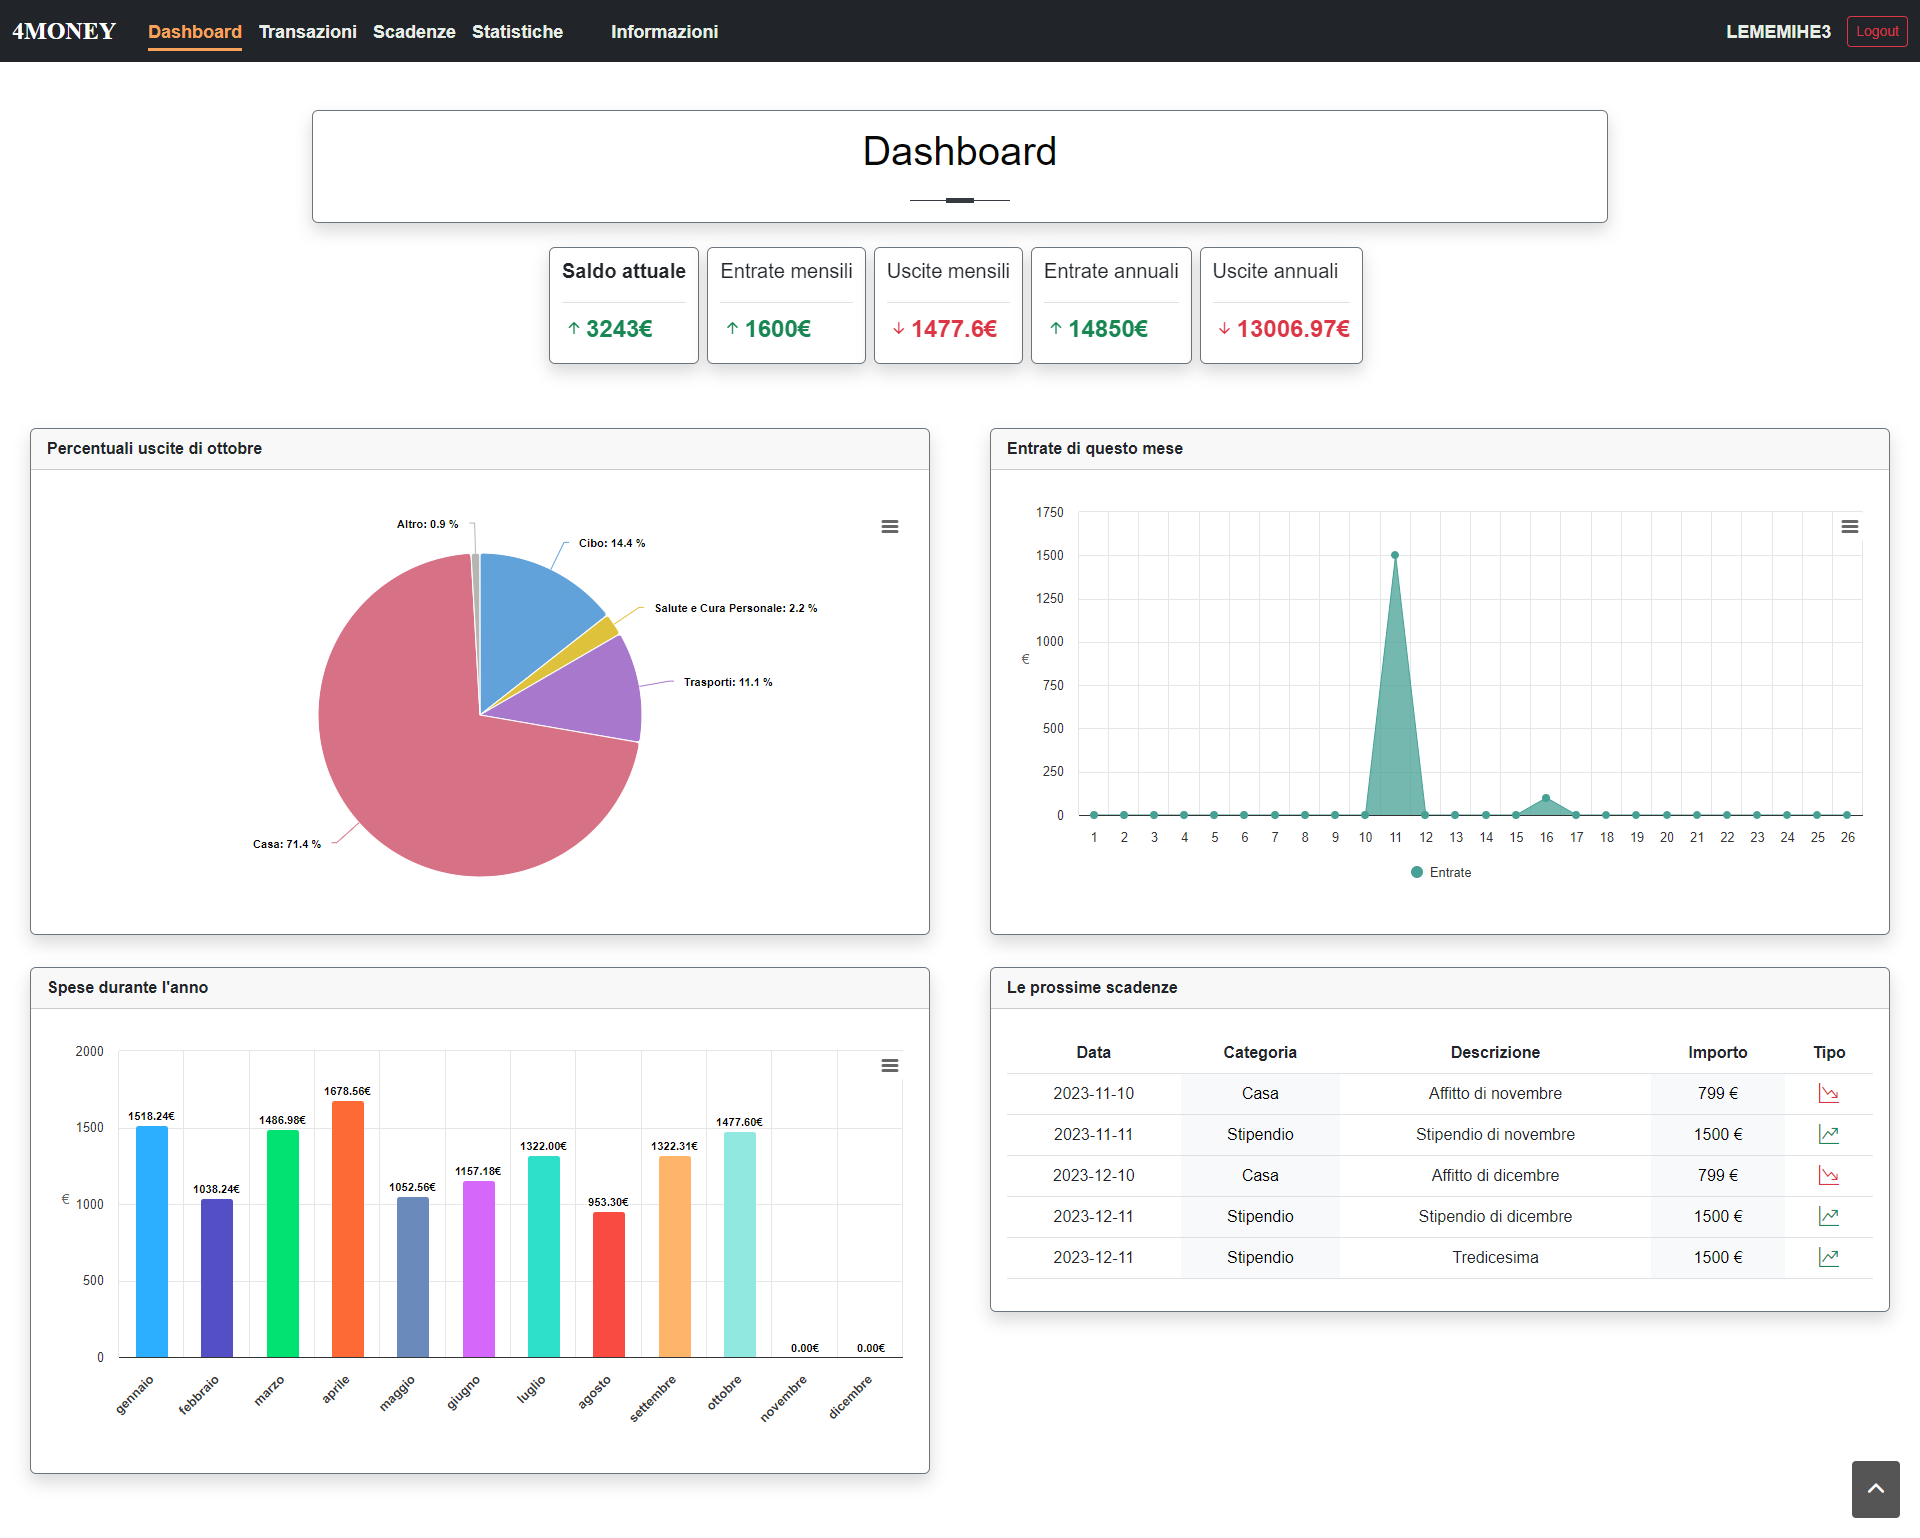
\includegraphics[width=1\linewidth]{dashboard.png}
    \caption{Pagina Dashboard}
    \label{fig:dashboard}
\end{figure}
Una volta avvenuto l'accesso da parte dell'utente, questo verrà indirizzato verso la pagina "Dashboard", cosiderata il cuore di 4Money, dove è possibile tenere sottocontrollo le principali informazioni che il sito fornisce. La pagina potrebbe essere definita in cinque sezioni:
\begin{enumerate}
    \item I cinque riquadri in alto mostrano informazioni quantitative sul saldo attuale dell'utente, oltre che sulle entrate e sulle uscite del mese e dell'anno in corso. Questi numeri vengono calcolati basandosi sulle transazioni inserite dall'utente e sul saldo iniziale inserito in fase di registrazione;
    \item Sotto i riquadri a sinistra è presente il primo dei tre grafici della pagina realizzati con Highcharts. In particolare, questo è un grafico a torta che mostra le percentuali delle spese del mese in corso in base alla categoria. In questo modo l'utente si può rendere conto quale sia la categoria che è gli è costata maggiormente durante il mese.
    \item Alla destra del grafico a torta è presente uno a linea, che mostra la variazione delle entrate durante i giorni del mese corrente;
    \item In basso a sinistra vi è un grafico a colonne che indica il valore delle spese durante l'anno corrente per ogni mese;
    \item Infine, in basso a destra, è presente una tabella che indica le imminenti scadenze delll'utente, da lui precedentemente inserite, fungendo da promemoria per esso.
\end{enumerate}
Osserviamo ora l'implementazione di uno dei grafici con Highcharts, il cui codice viene mostrato nella figura 2.9. \\
\begin{figure}[h]
    \centering
    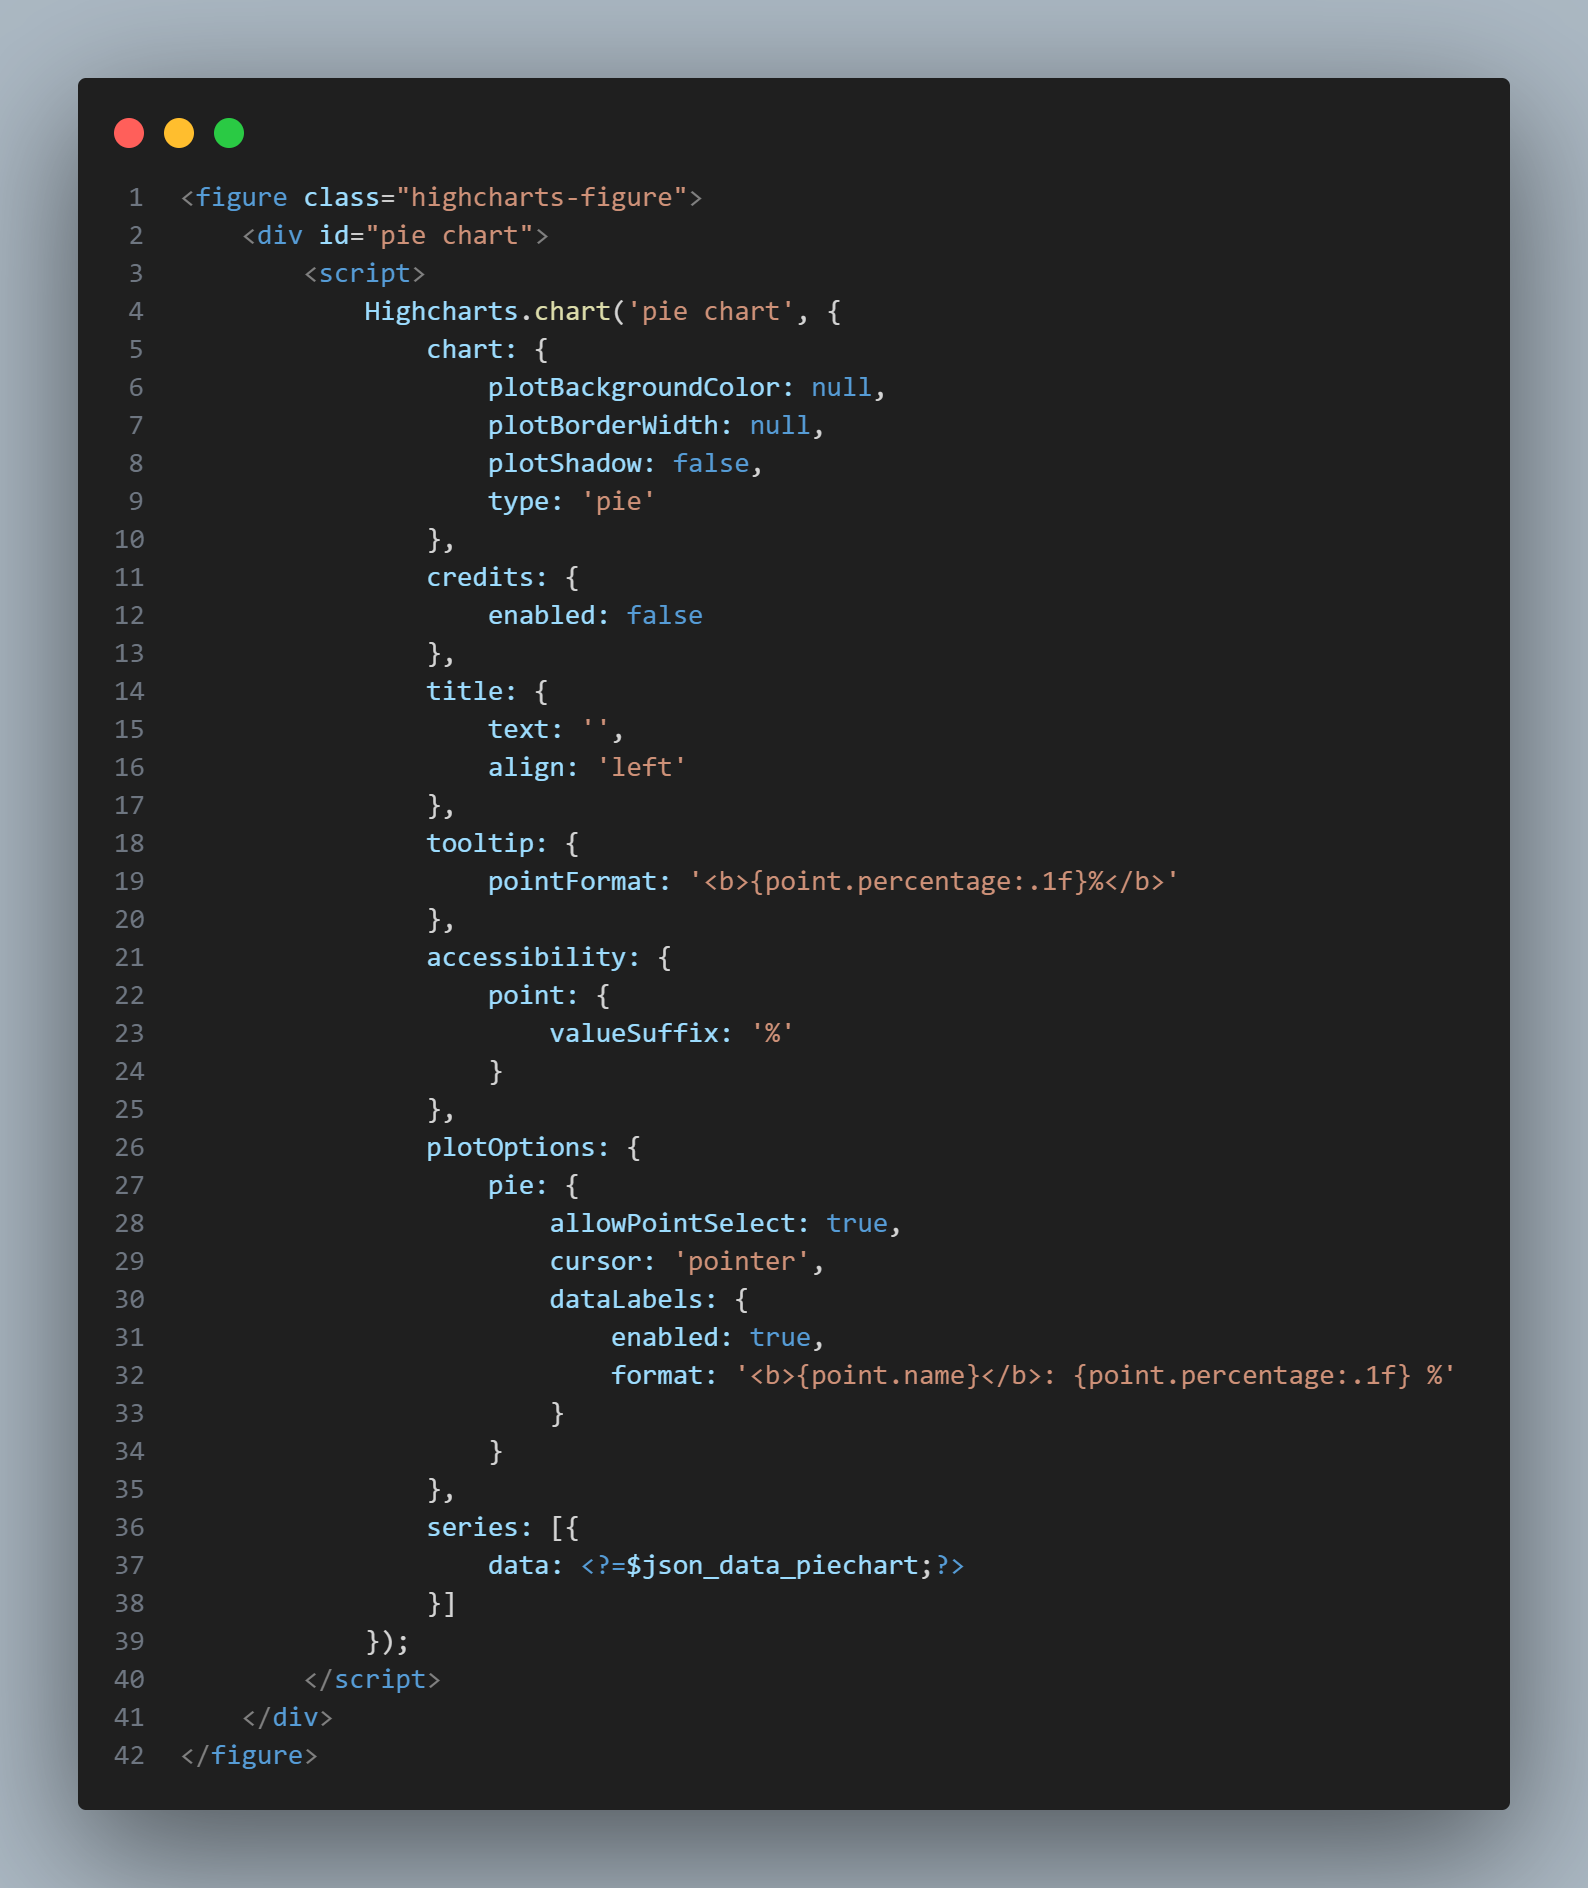
\includegraphics[width=1\linewidth]{piechart_code.png}
    \caption{Codice del grafico a torta}
    \label{fig:piechart_code}
\end{figure} \\
Il codice si presenta come un comune script di JavaScript, costruendo un oggetto "Highcharts.chart" in base al nome inserito, nel nostro caso "pie chart", e alla compilazione dei vari attributi del grafico, come il titolo o il formato delle etichette delle sezioni, ma l'attributo di maggiore importanza è "series": andranno, infatti, inseriti qui i dati che devono essere inseriti nel grafico, in formato Json. Nel caso del grafico a torta i dati da inserire richiedono un nome, il nome della categoria per quello della pagina "Dashboard", un colore da assegnare alla sezione di quel dato e la percentuale da dedicare alla sezione. \\
\MakeUppercase{è} necessario far notare che i dati mostrati dai grafici fanno riferimento al mese o anno fino al giorno attuale in cui vengono visualizzati e non a questi nella loro completezza. Si osserva facilmente infatti che il grafico a linea presenta informazioni fino al giorno 26, mentre il grafico a colonne fino al mese di ottobre, data in cui sono state salvate le schermate delle figure presenti in questa tesi.
\newpage
\subsection{Transazioni}
\begin{figure}[h]
    \centering
    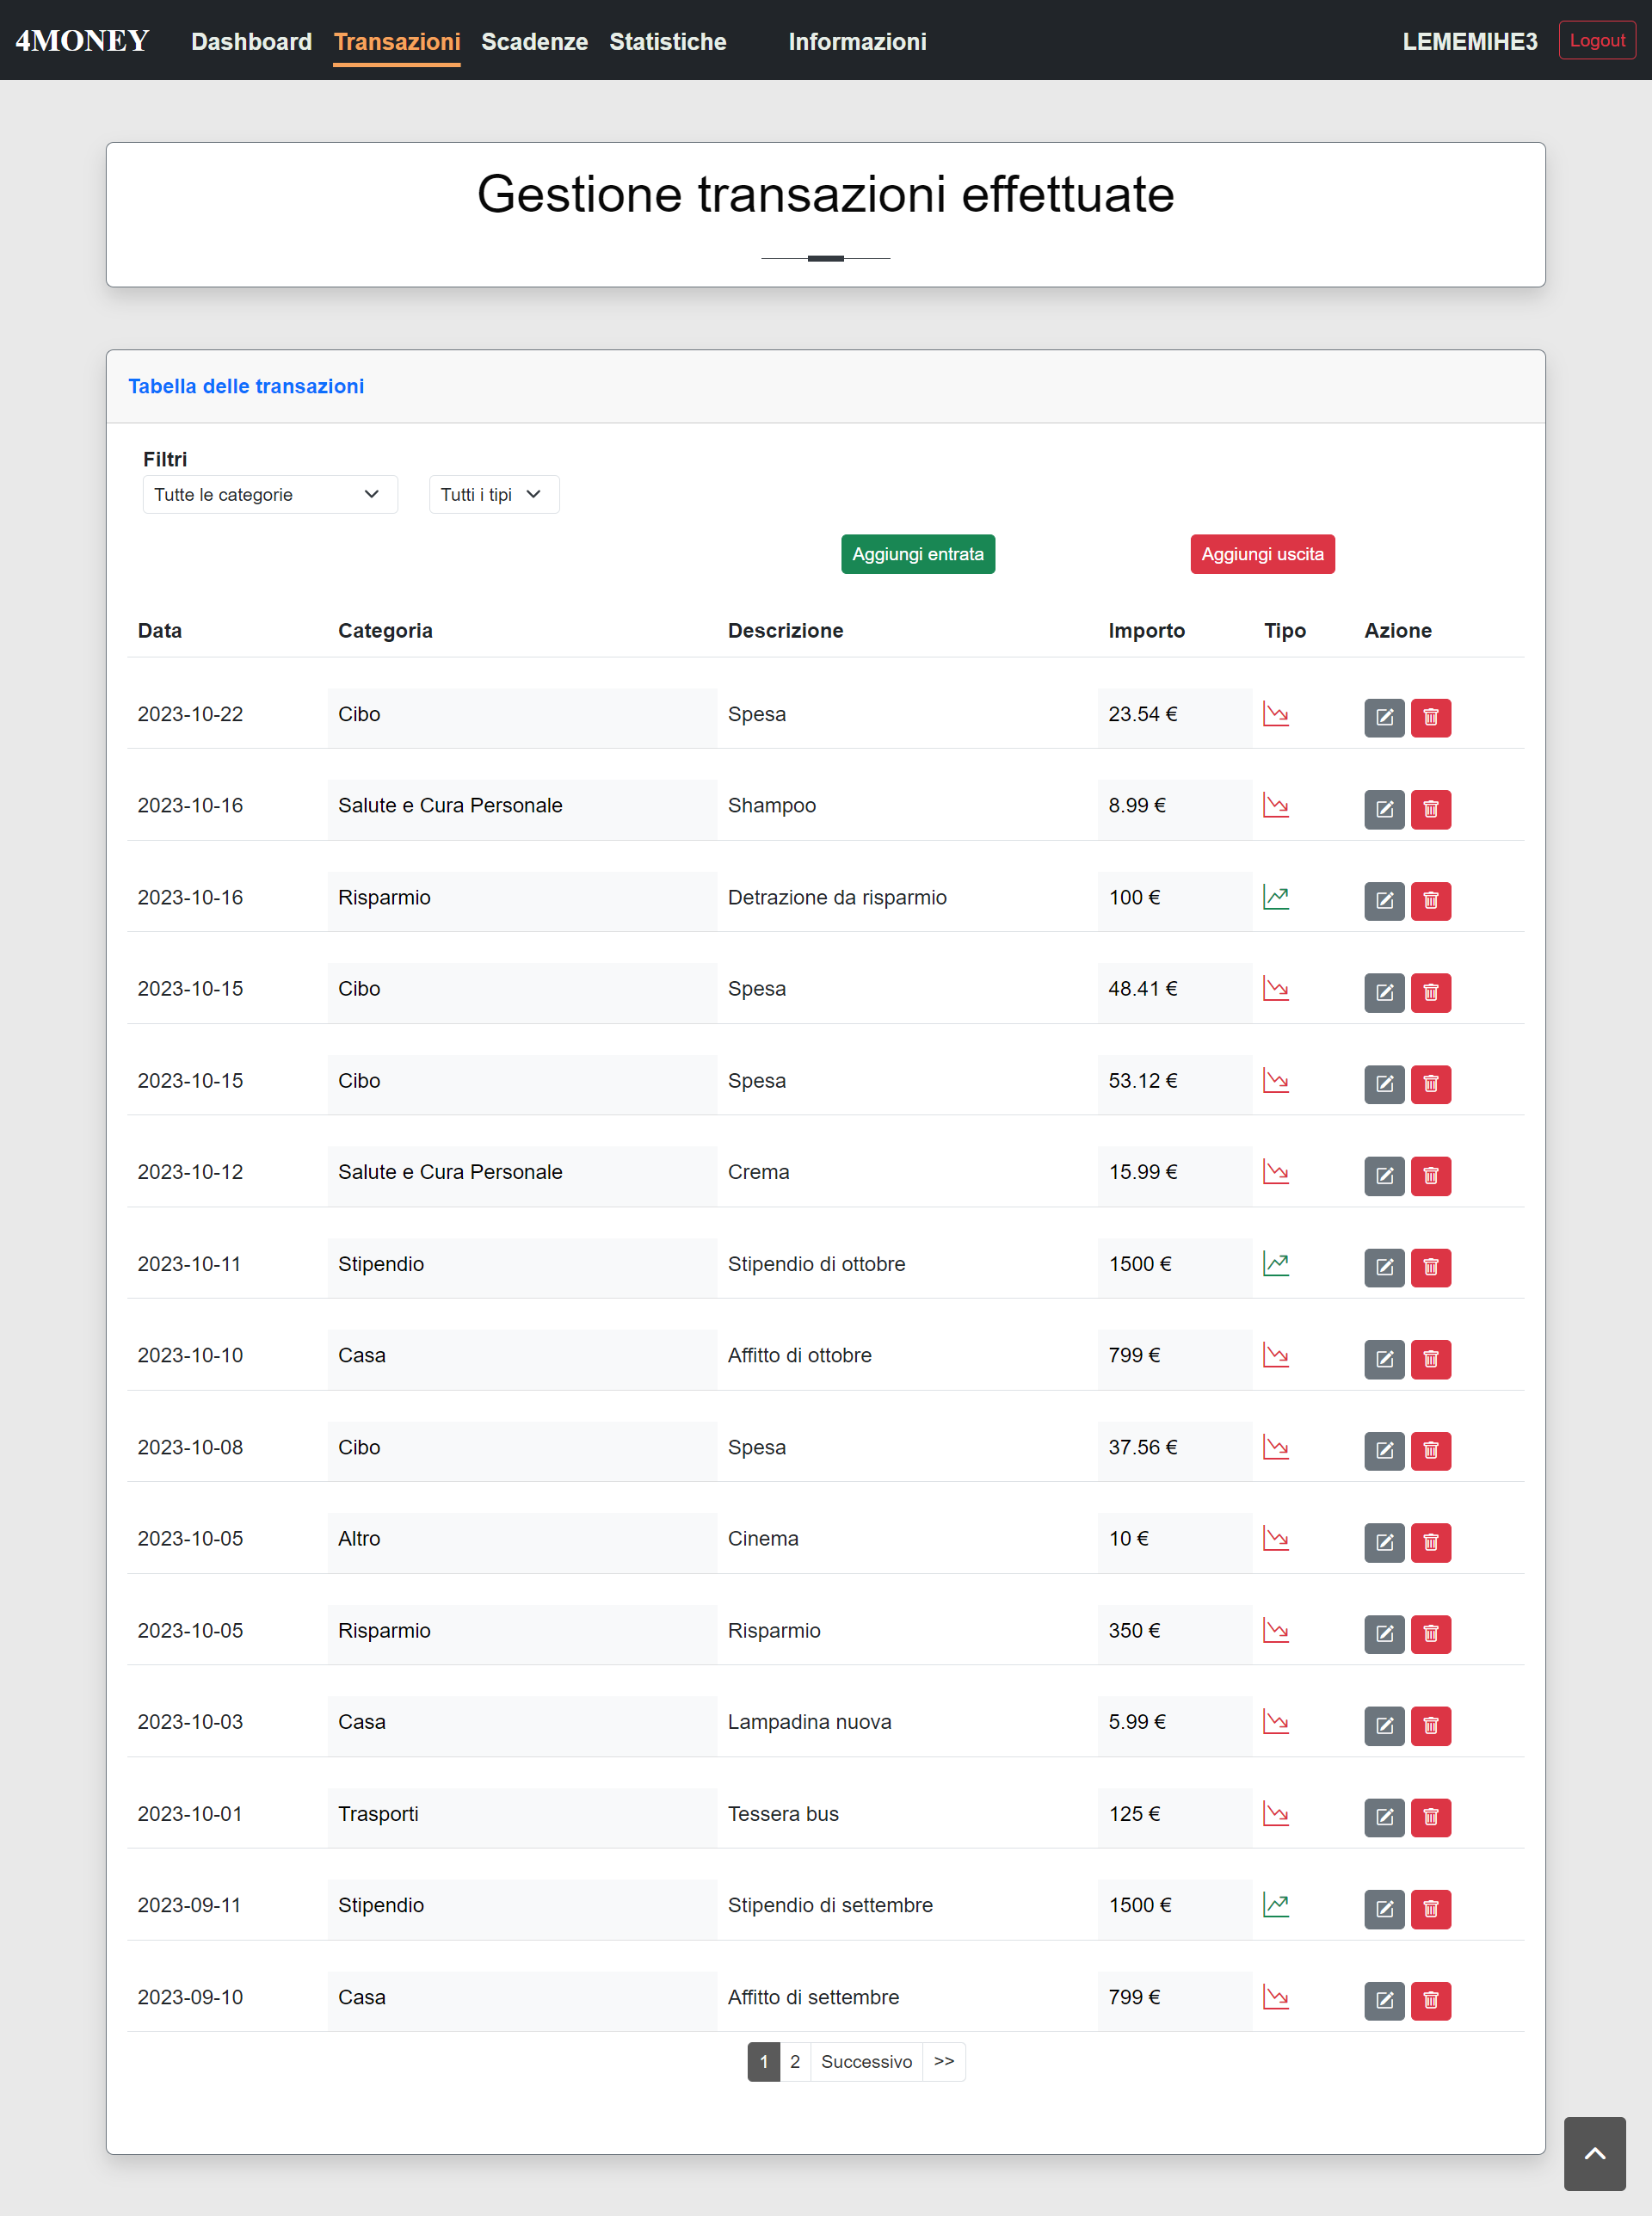
\includegraphics[width=0.85\linewidth]{transazioni.png}
    \caption{Pagina delle transazioni}
    \label{fig:transazioni}
\end{figure}
La pagina "Transazioni" è la pagina dedita alla registrazione delle varie spese affrontatate dall'utente, nonché eventuali entrate. Queste vengono visualizzate come righe di una tabella in ordine cronologico, dove le righe più in alto indicano le più recenti transazioni. L'utente può interagire con la tabella in diversi modi:
\begin{itemize}
    \item Attraverso i filtri, costituiti da due pulsanti a finestra dove è possibile selezionare la categoria ed il tipo, ovvero se la transazione è una spesa o un introito, di interesse. L'implementazione dei filtri è stata fatta con AJAX per evitare di dover caricare nuovamente la pagina ogni volta che si utilizza un filtro, in quanto l'utente potrebbe voler fare questa operazione numerose volte e questo permette una maggiore rapidità nell'esecuzione di tale azione;
    \item Attraverso pulsanti quali "Aggiungi entrata" ed "Aggiungi uscita", che permettono come suggerisce il nome di aggiungere una transazione del corrispettivo tipo, aprendo una sottofinestra detta "modal", di cui discuteremo successivamente
    \item Attraverso i pulsanti presenti alla destra di ogni transazione: il punsate grigio apre un modal simile a quello di registrazione delle transazioni, ma questo serve per modificare i dati della riga corrispondente; il pulsante rosso serve invece ad eliminare tale transazione.
    \item Attraverso una barra di navigazione, che non ha nulla a che fare con la navbar, che si trova in fondo alla pagina. Questa permette di visualizzare altre transazioni oltre alle 20 presenti nella tabella, organizzate in ordine cronologico. Si può passare da una tabella alla precedente o successiva, o, in alternativa, verso la prima o ultima. Anche questa funzione è stata implementata con AJAX per rendere più dinamica questa operazione
\end{itemize}
Nella figura 2.11 si può osservare un esemopio di uno dei modal della pagina "Transazioni". \\
\begin{figure}[h]
    \centering
    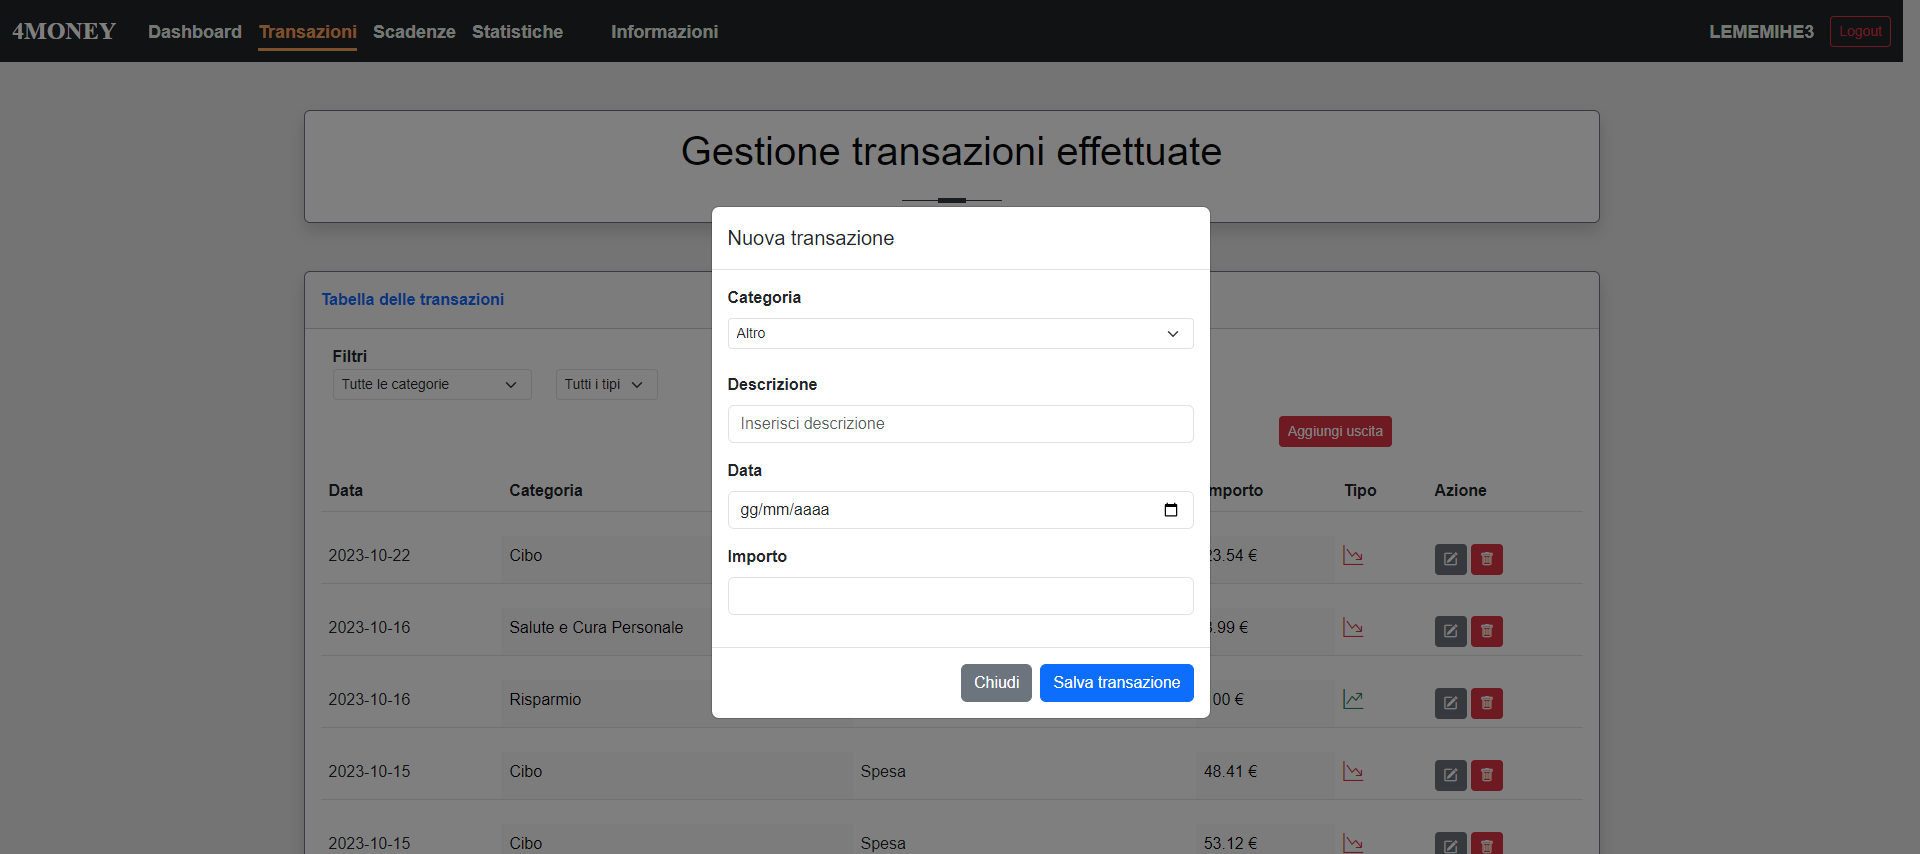
\includegraphics[width=1\linewidth]{modal_transazioni.png}
    \caption{Modal delle transazioni}
    \label{fig:modal_transazioni}
\end{figure} \\
Il modal qui esaminato è quello generato dal click sul pulsante "Aggiungi uscita", ma gli altri sono identici se non per l'inizializzazione dei campi nel modal di modifica. Questa sottofinestra contiene un form che richiede delle informazioni sulla transazione: inizialmente è presente un pulsante a scorrimento per la selezione della categoria tra quelle esistenti nel sistema; a seguire si ha un campo di testo dove inserire una descrizione, per poter aggiungere informazioni più dettagliate nel caso la categoria non basti a specificare le ragioni dietro quella transazione; si devono poi selezionare una data e un importo. Quest'ultimo deve essere un numero decimale o un intero, nel qual caso sarà considerato come un numero decimale con nessuna cifra decimale e quindi nessun centesimo. Non bisogna specificare il segno dell'importo, visto che questo verrà trattato di corrispondenza in base al tipo di modal in cui è stato inserito. I pulsanti "Salva transazione" e "Chiudi" servono rispettivamente a confermare l'invio del form oppure ad annullare l'operazione. In seguito all'inserimento della transazione nel sistema verrà inivato a schermo un messaggio di errore o di successo a seconda del risulatato dell'azione.
\subsection{Scadenze}
\begin{figure}[h]
    \centering
    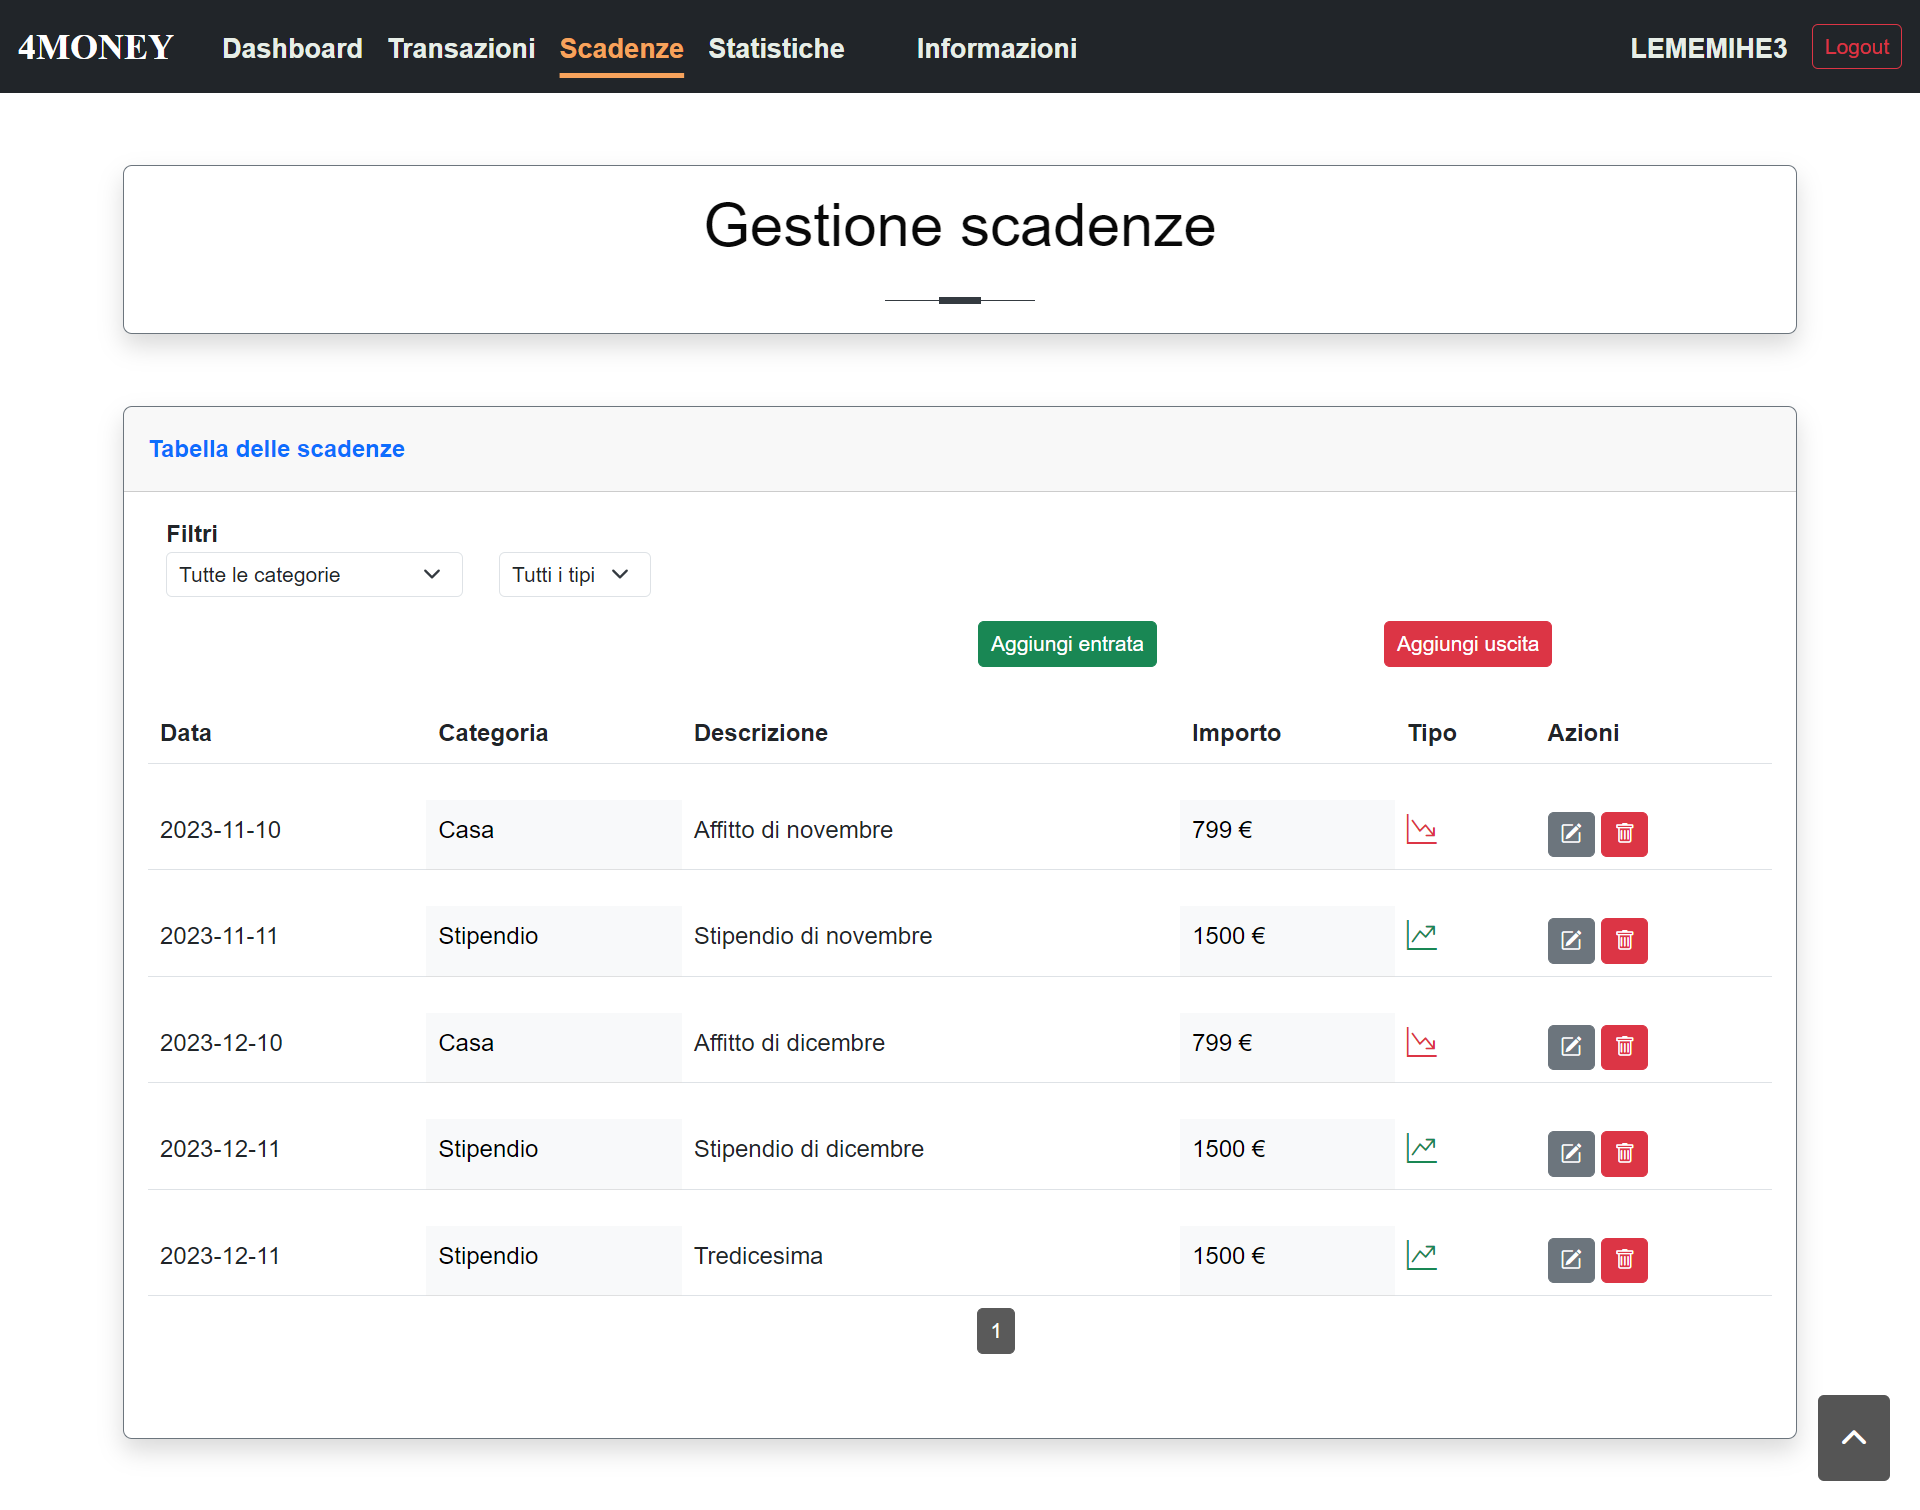
\includegraphics[width=1\linewidth]{scandenze.png}
    \caption{Pagina delle scadenze}
    \label{fig:scadenze}
\end{figure}
La pagina "Scadenze" è del tutto identica alla pagina "Transazioni" in aspetto e funzionalità, ma introduce un nuovo concetto: quello appunto di scadenza. Per scadenza si intende una transazione che non è ancora avvenuta ed è stata inserita in una data futura. Una particolarità che questo concetto ha portato è stata il modo in cui viene trattato il dato "data" dei modal delle transazioni e delle scadenze stesse: a seconda della data inserita il sistema riconoscerà in automatico a quale delle due appartiene e verrà inserita nella corrispodente tabella, indirizzando l'utente verso l'omonima pagina al completamento dell'operazione.
\newpage
\subsection{Statistiche}
\begin{figure}[h]
    \centering
    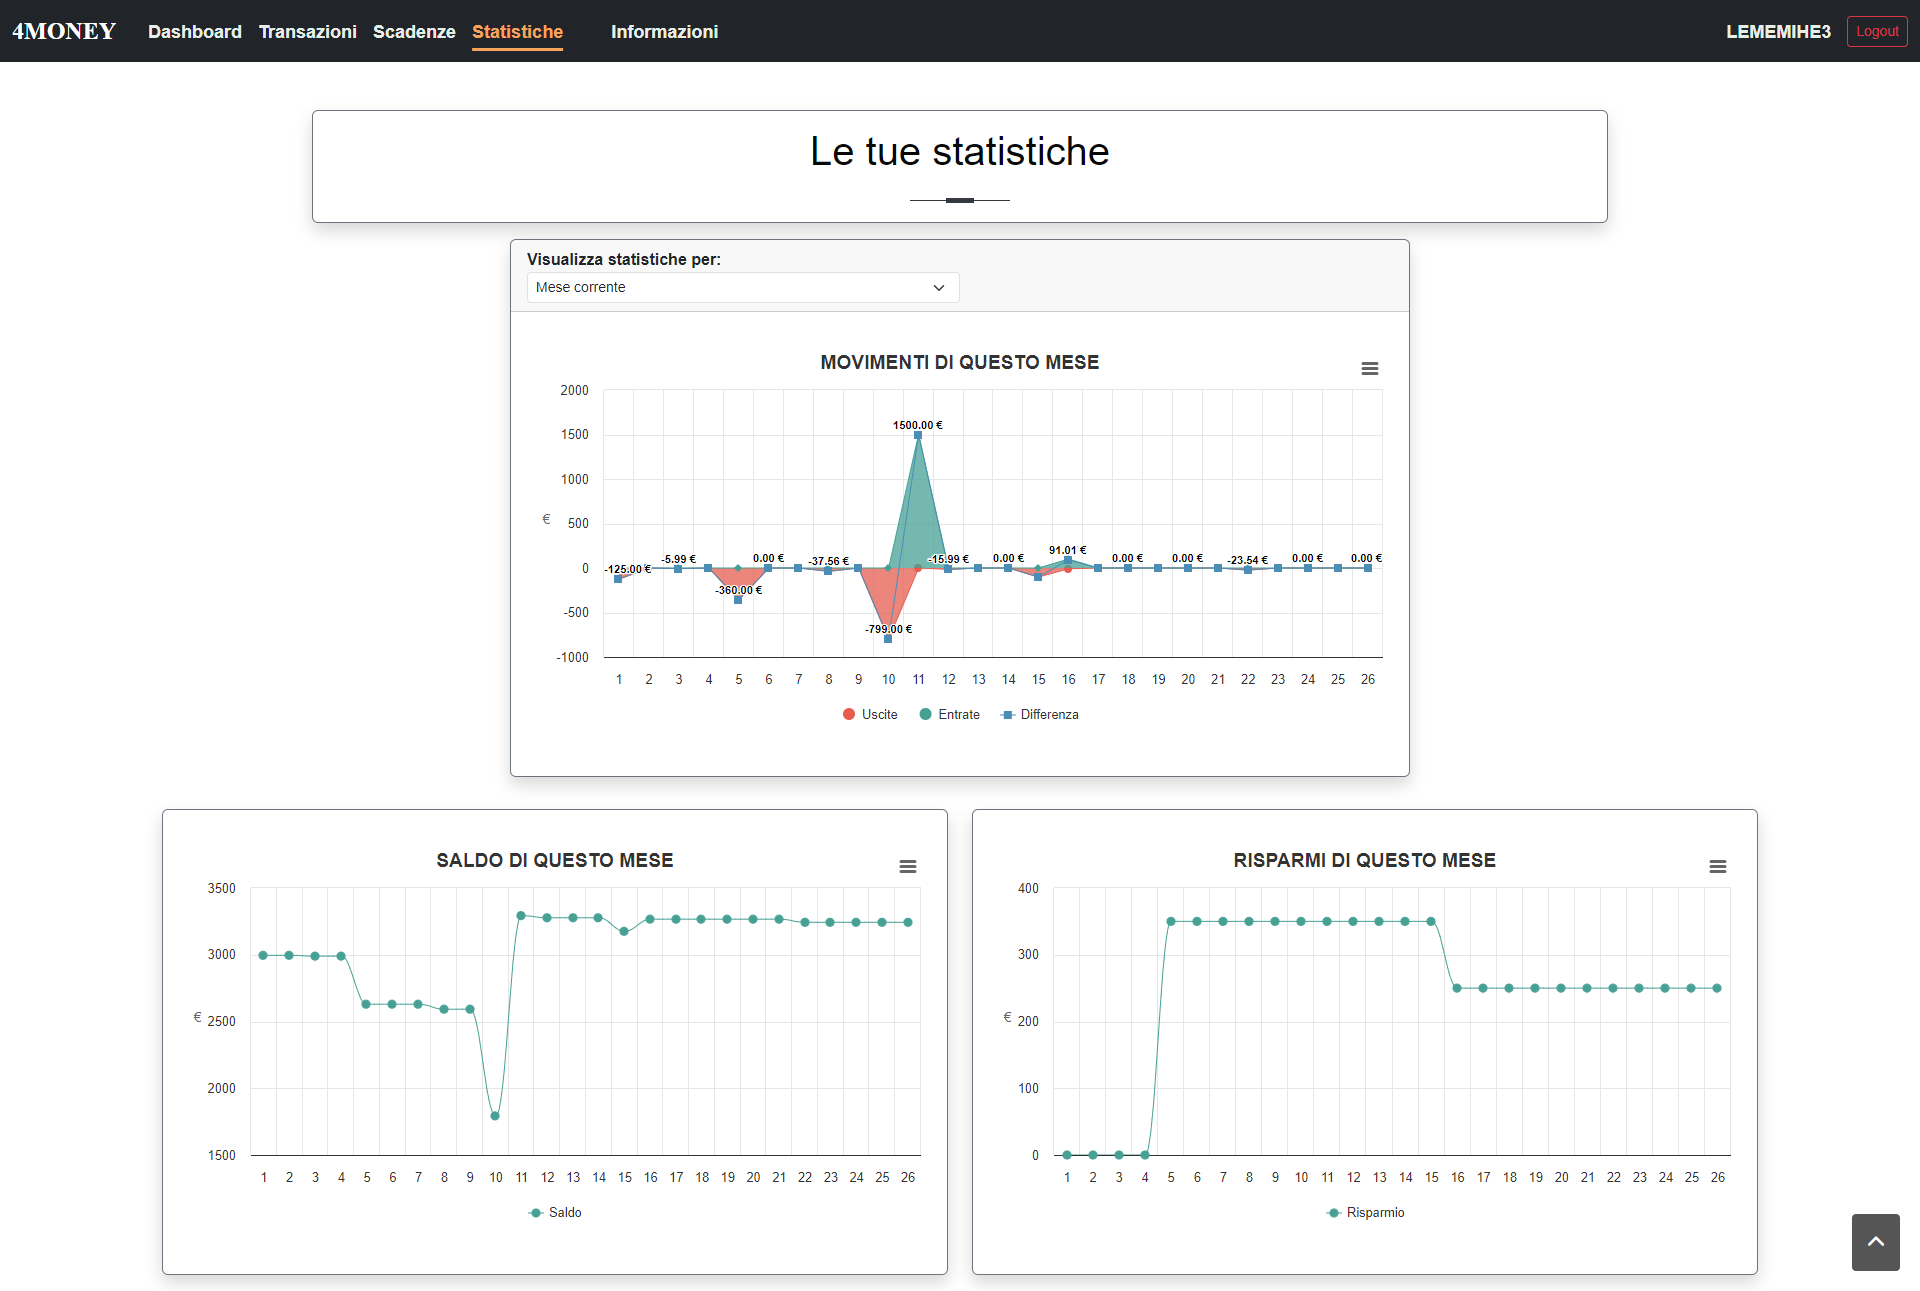
\includegraphics[width=1\linewidth]{statistiche.png}
    \caption{Pagina delle statistiche}
    \label{fig:statistiche}
\end{figure}
La pagina "Statistiche" presenta dei grafici di particolare interesse per l'utente nella gestione delle proprie finanze, senza essere caretterizzati dall'essenzialità di quelli presenti nella dashboard. In particolare la pagina presenta tre grafici e un pulsante che modifica il periodo di riferimento di quest'ultimi, in quanto normalemente la visulizzazione avviene per il mese corrente, ma è possibile selezionare come periodo anche l'anno in corso.
\begin{itemize}
    \item Il grafico in alto è un misto tra grafico a linee ed ad area: le aree verdi e rosse rappresentano rispettivamente il valore delle entrate e delle uscite, mentre la linea azzurra mette in evidenza la differenza tra le precedenti. L'utente è così in grado di comprendere la distribuzione durante il mese o l'anno di come esso ricava o spende il proprio denaro;
    \item Il grafico in basso a sinistra indica l'andamento del saldo nel corso del mese o anno di riferimento, dando modo all'utente di comprendere se esso è mai stato in crisi finanziarie oppure ha mantenuto un comportamento costante. Il calcolo dei valori del grafico dipendono dalle transazioni del periodo di riferimento, in particolare, il primo valore del periodo è lo stesso dell'ultimo del periodo precedente e viene calcolato in base a tutte le transazioni e al saldo iniziale dichiarato. Inoltre il colore del grafico dipende dal segno dell'ultimo valore disponibile: se questo è positivo la linea sarà di colore verde, come da figura, altrimenti, nel caso di un saldo negativo, la linea divernterà rossa, fungendo da indicatore di pericolo per l'utente che osserva tale grafico;
    \item Il grafico in basso a destra, in modo simile al precedente, indica l'andamento del "Risparmio" durante il periodo di riferimento. Per risparmio si intende una particolare categoria nel modo in cui questa viene trattata. A seconda del tipo di transazione che ha "risparmio" come categoria il saldo si comporterà in modo diverso: se sto segnando una spesa allora questa verrà considerata come un decremento per il saldo ed un incremento per il risparmio, al contrario, un entrata è considerata un incremento del saldo ed un decremento per il risparmio. Lo scopo di questa funzione è di permettere all'utente di poter gestire un conto di risparmio aiutando l'utente a "salvare" i propri soldi. Anche questo grafico cambia colore in base al segno dell'ultimo valore disponibile.
\end{itemize}
\subsection{Profilo utente}
\begin{figure}[h]
    \centering
    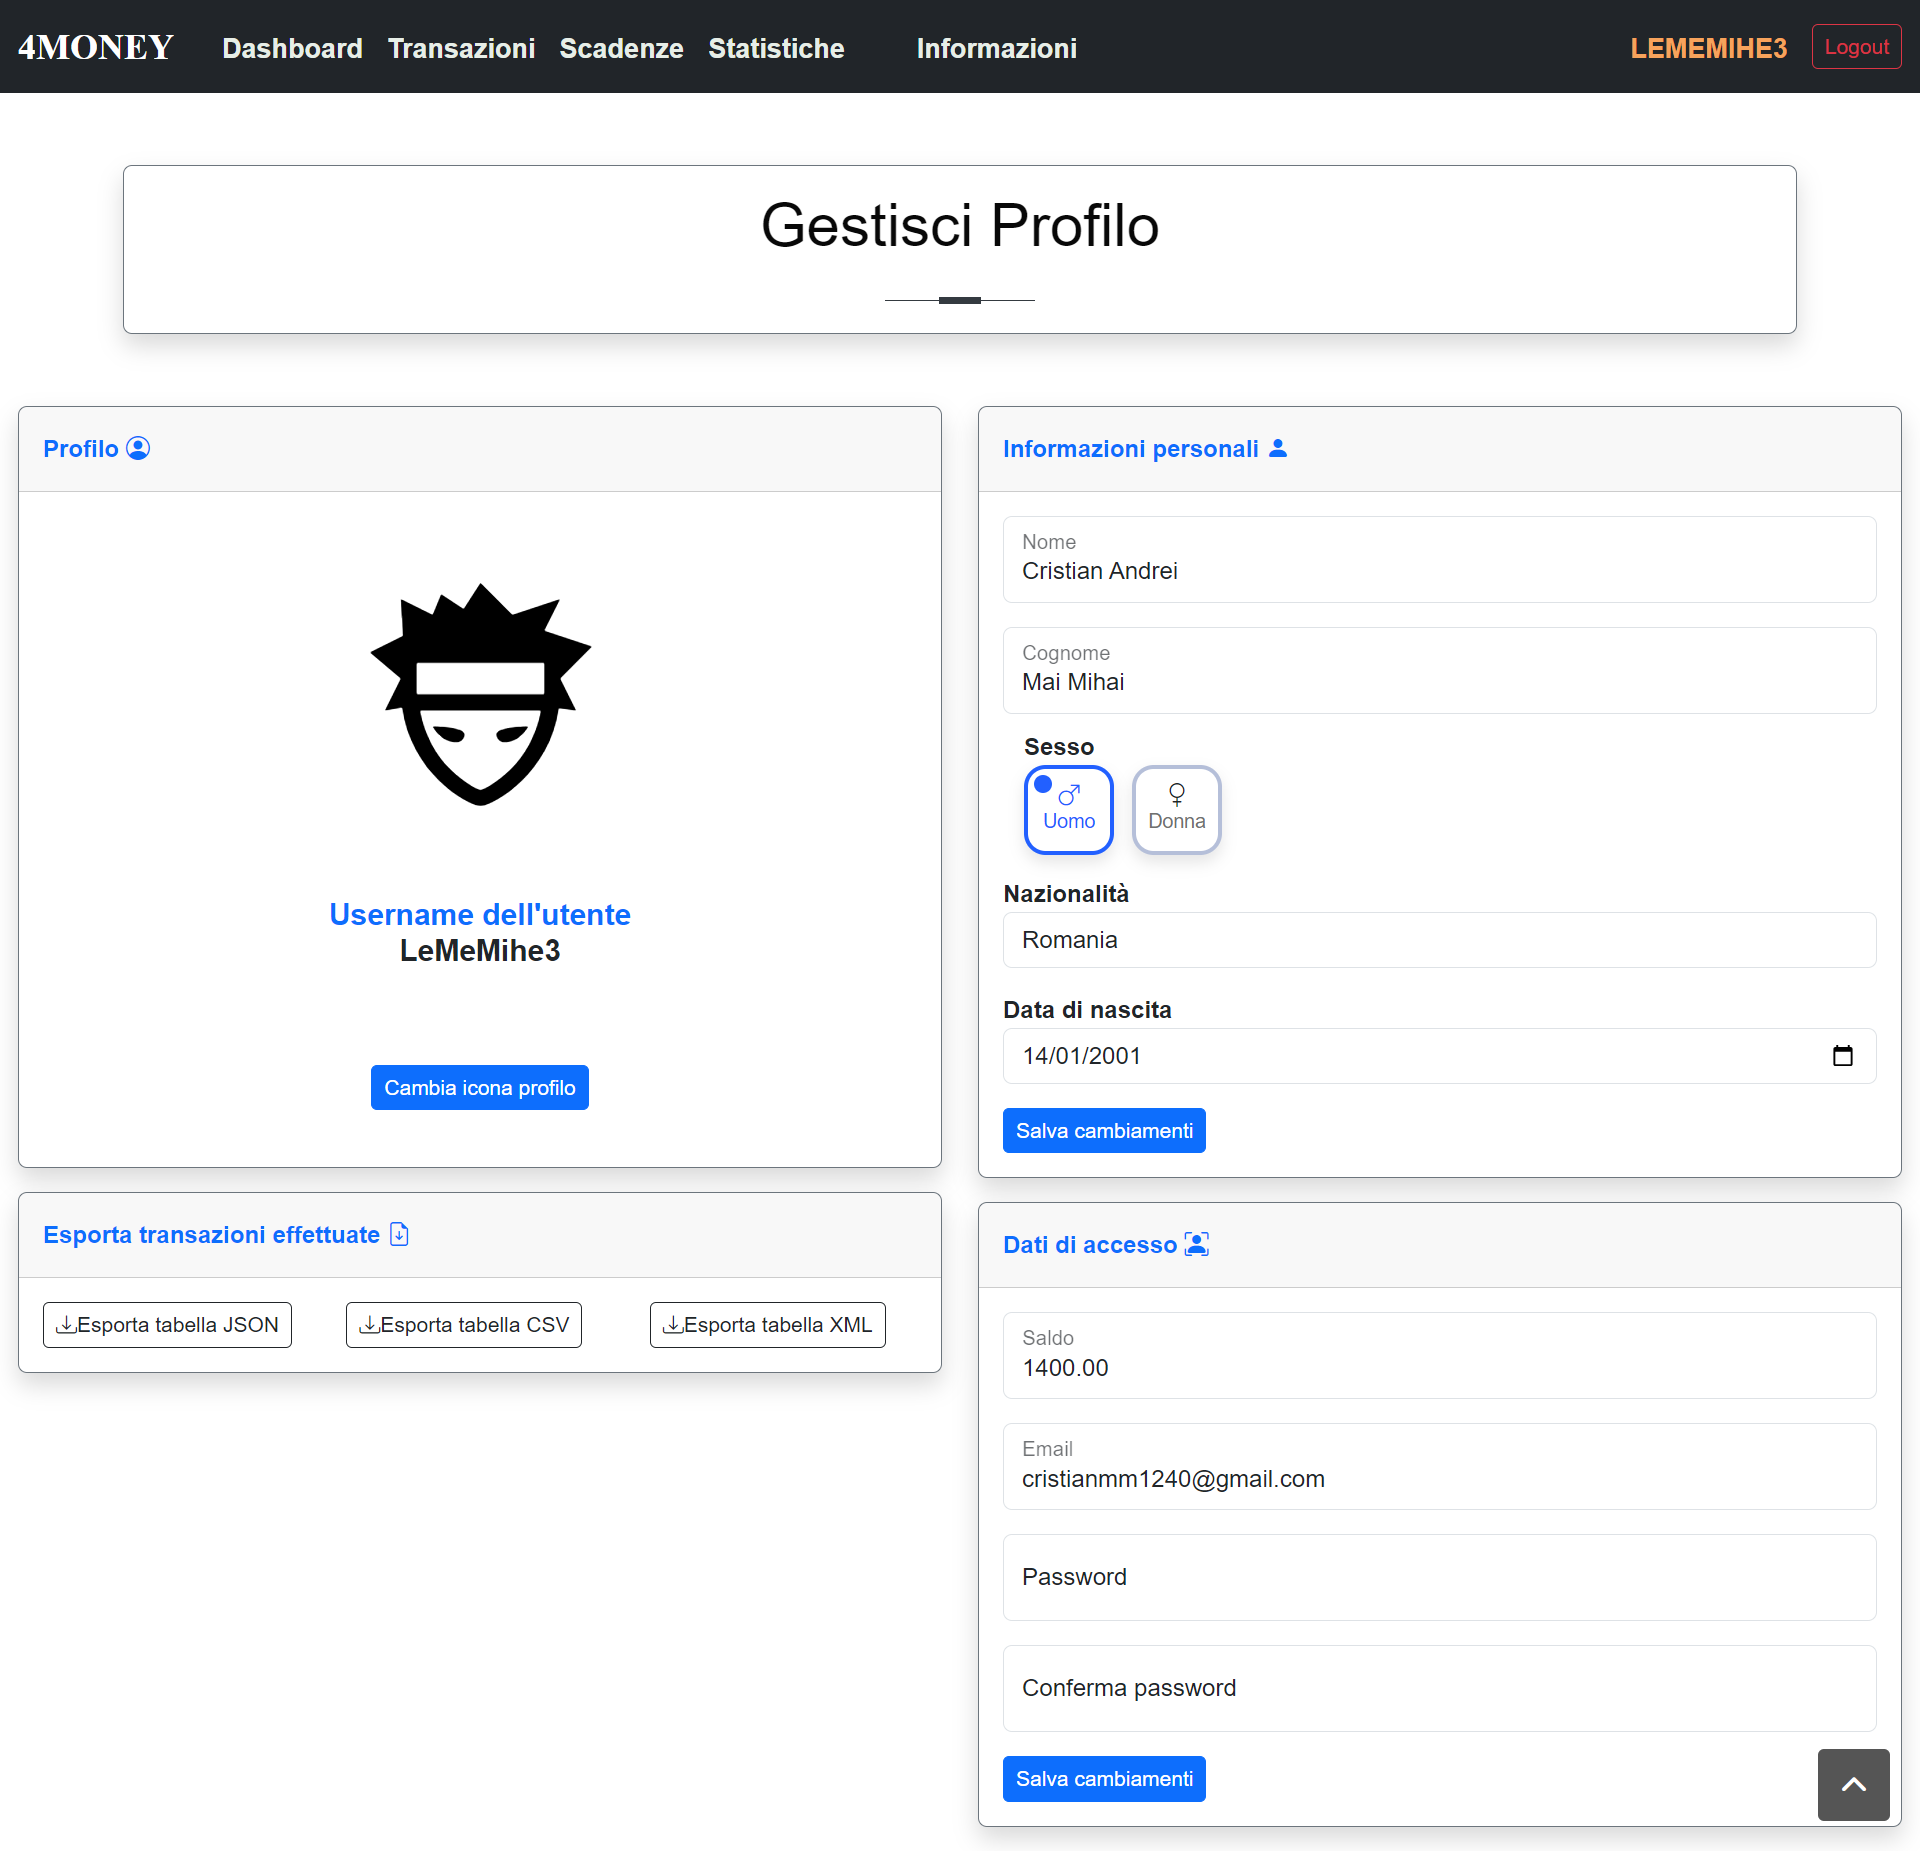
\includegraphics[width=1\linewidth]{profile.png}
    \caption{Pagina del profilo utente}
    \label{fig:profile}
\end{figure}
La pagina "Profilo" è la pagina nella quale l'utente può visualizzare le informazioni riguardanti il proprio profilo inserite in fase di registrazione. L'interfaccia si presenta divisa in 4 sezioni di interesse:
\begin{itemize}
    \item In alto a sinistra la sezione "Profilo", dove vengono mostrati l'username e l'immagine di profilo, la quale può essere modificata, ma selezionata solo tra quelle predefinite dal sito;
    \item In basso a sinistra la sezione "Esporta transazioni effettuate". Qui sono tre presenti tre pulsanti che permettono, come suggerisce il loro nome, di scaricare le informazioni della tabella della pagina "Transazioni" in diversi formati: Json, CSV e XML;
    \item In alto a destra la sezione "Informazioni personali", composta da un form dove è possibile modificare i dati personali dell'utente;
    \item In basso a destra la sezione "Dati di accesso", anche questa composta da un form del tutto indipendente dal precedente, dove è possibile modificare le informazioni strattamente riguardanti l'account. Nel caso in cui attraverso questa sezione venga modificata la password l'utente sarà disconnesso in automatico e dovrà effettuare nuovamente l'accesso, questa volta utilizzando la nuova password.
\end{itemize}
\subsection{Utenti}
\begin{figure}[h]
    \centering
    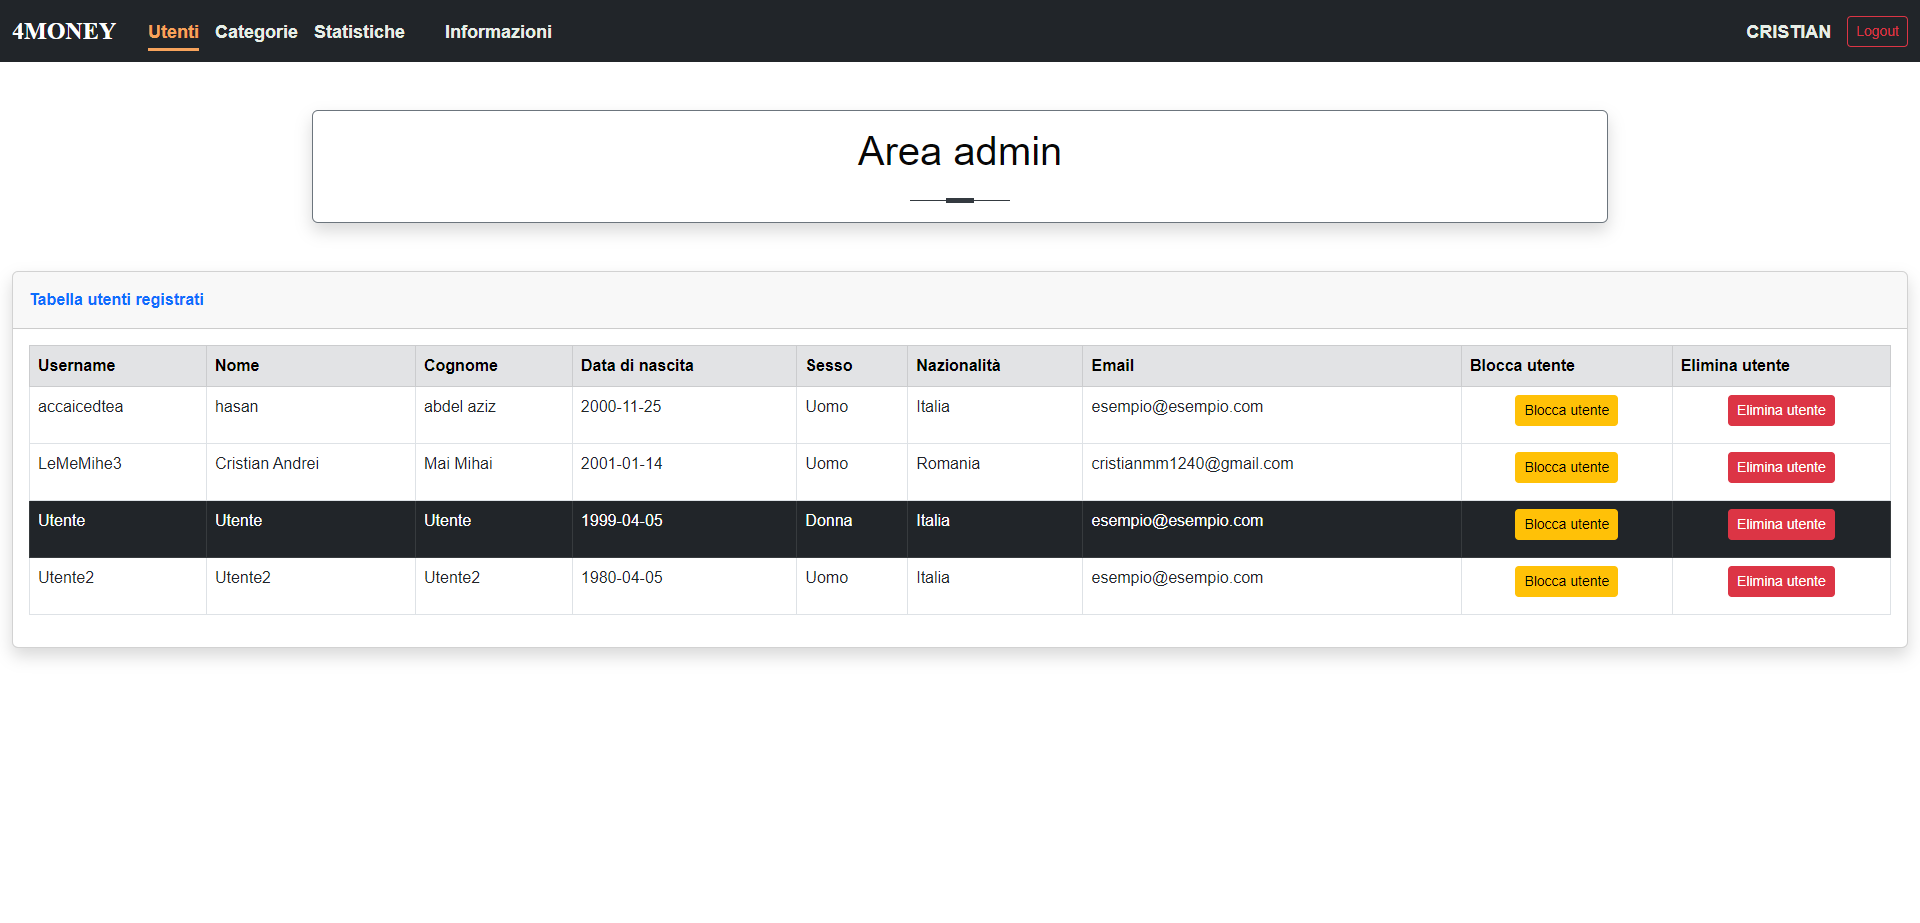
\includegraphics[width=1\linewidth]{utenti_admin.png}
    \caption{Pagina degli utenti}
    \label{fig:utenti_admin}
\end{figure}


\end{document}
